% ============================================================================
% Physics (Economics)-Informed Neural Networks (PINNs)
% Summer School on AI for Economics and Finance
% ESOMAS, University of Torino, August 25, 2026
% Duration: 90 minutes
% ============================================================================

\documentclass[aspectratio=169,11pt]{beamer}

% ---------- Theme and colors ----------
\usecolortheme{dove}
\setbeamertemplate{navigation symbols}{}
\setbeamertemplate{footline}{%
  \hfill\usebeamerfont{page number in head/foot}%
  \usebeamercolor[fg]{normal text}%
  \insertframenumber\,/\,\inserttotalframenumber\kern1em\vskip4pt}
\setbeamerfont{frametitle}{size=\huge}

% ---------- Packages ----------
\usepackage[utf8]{inputenc}
\usepackage[T1]{fontenc}
\usepackage{amsmath,amssymb,amsfonts}
\usepackage{bm}
\usepackage{graphicx}
\usepackage{tikz}
\usetikzlibrary{shapes,arrows.meta,positioning,calc,fit,backgrounds,patterns,decorations.pathreplacing}
\usepackage{pgfplots}
\pgfplotsset{compat=1.18}
% --- readable-from-the-back defaults for every plot ---
\pgfplotsset{every axis/.append style={
    tick label style={font=\footnotesize},
    label style={font=\small},
    title style={font=\small},
    legend style={font=\footnotesize}}}
\usepgfplotslibrary{fillbetween}
\usepackage{booktabs}
\usepackage{hyperref}
\usepackage{multicol}
\usepackage{xcolor}
\usepackage{algorithm}
\usepackage{algorithmic}
\usepackage{array}
\usepackage{listings}

% ---------- Tighter display math, applied uniformly at every font size ------
% (a global typographic setting, so that no frame needs a local \vspace hack)
\makeatletter
\g@addto@macro\normalsize{%
  \setlength\abovedisplayskip{5pt plus 2pt minus 2pt}%
  \setlength\belowdisplayskip{5pt plus 2pt minus 2pt}%
  \setlength\abovedisplayshortskip{2pt plus 1pt}%
  \setlength\belowdisplayshortskip{3pt plus 1pt}}
\g@addto@macro\small{%
  \setlength\abovedisplayskip{4pt plus 2pt minus 2pt}%
  \setlength\belowdisplayskip{4pt plus 2pt minus 2pt}%
  \setlength\abovedisplayshortskip{2pt plus 1pt}%
  \setlength\belowdisplayshortskip{2pt plus 1pt}}
\g@addto@macro\footnotesize{%
  \setlength\abovedisplayskip{3pt plus 2pt minus 2pt}%
  \setlength\belowdisplayskip{3pt plus 2pt minus 2pt}%
  \setlength\abovedisplayshortskip{1pt plus 1pt}%
  \setlength\belowdisplayshortskip{2pt plus 1pt}}
\makeatother

% ---------- Custom colors ----------
\definecolor{uzhblue}{rgb}{0,0,0.5}
\definecolor{uzhgreylight}{RGB}{236,238,241}
\definecolor{uzhgreydark}{RGB}{81,86,94}
\definecolor{harvardcrimson}{RGB}{153,0,0}
\definecolor{unil@blue}{RGB}{0,140,204}
\definecolor{unil@black}{RGB}{35,31,32}
\definecolor{darkgreen}{RGB}{0,100,0}
\definecolor{darkred}{RGB}{139,0,0}
\definecolor{softblue}{RGB}{70,130,180}
\definecolor{softorange}{RGB}{230,159,0}
\definecolor{softgreen}{RGB}{0,158,115}

% ---------- Listings style for Python ----------
% (defined after the colours it references, so the style is not held together
%  by lstset's deferred token expansion)
\lstset{
    language=Python,
    basicstyle=\small\ttfamily,
    keywordstyle=\color{uzhblue}\bfseries,
    commentstyle=\color{uzhgreydark}\itshape,
    stringstyle=\color{darkgreen},
    showstringspaces=false,
    breaklines=true,
    breakatwhitespace=true,
    columns=fullflexible,
    frame=none,
    xleftmargin=0pt,
    aboveskip=4pt,
    belowskip=4pt,
    escapeinside={(*@}{@*)},
}

% ---------- Set beamer colors ----------
\setbeamercolor{frametitle}{bg=uzhgreylight, fg=uzhblue}
\setbeamercolor{title}{fg=uzhblue}
\setbeamercolor{structure}{fg=uzhblue}
\setbeamercolor{block title}{bg=unil@blue, fg=white}
\setbeamercolor{block body}{bg=uzhgreylight}
\setbeamercolor{block title alerted}{bg=darkred,fg=white}
\setbeamercolor{block body alerted}{bg=red!5}
\setbeamercolor{block title example}{bg=darkgreen,fg=white}
\setbeamercolor{block body example}{bg=green!5}
\setbeamercolor{item}{fg=unil@black}
\setbeamercolor{normal text}{fg=unil@black}

% ---------- Emphasis and hyperlinks ----------
\newcommand{\emphc}[1]{\textcolor{harvardcrimson}{#1}}
\hypersetup{colorlinks,linkcolor=harvardcrimson,urlcolor=harvardcrimson}

% ---------- Math commands ----------
\newcommand{\x}{\bm{x}}
\newcommand{\w}{\bm{w}}
\newcommand{\bb}{\bm{b}}
\newcommand{\z}{\bm{z}}
\newcommand{\W}{\bm{W}}
\newcommand{\X}{\bm{X}}
\renewcommand{\a}{\bm{a}}
\newcommand{\R}{\mathbb{R}}
\newcommand{\E}[1]{\mathbb{E}\!\left[#1\right]}
\DeclareMathOperator*{\argmin}{arg\,min}
\DeclareMathOperator*{\argmax}{arg\,max}

% ---------- Title ----------
\title[PINNs -- Torino 2026]%
{Summer School on AI for Economics and Finance}
\subtitle{Physics (Economics)-Informed Neural Networks}
\author{Simon Scheidegger}
\institute[HEC Lausanne]{HEC, University of Lausanne\\[4pt]
{\footnotesize Based on Raissi, Perdikaris \& Karniadakis (2019), \emph{Journal of Computational Physics} 378, 686--707}}
\date{University of Torino\\August 25, 2026}

\begin{document}
% --- Exercise pause badge ---
\newcommand{\exercisepause}{%
  \tikz[baseline=(X.base)]{\node[fill=darkgreen!80!black, text=white,
  rounded corners=2pt, inner sep=3pt, font=\scriptsize\bfseries](X){PAUSE, 5 min};}}


% ============================================================================
% PART 0: TITLE & OUTLINE
% ============================================================================

% --- Slide 1: Title ---
{\setbeamercolor{background canvas}{bg=uzhgreylight}
\begin{frame}
\titlepage
\vspace{-0.6cm}
\begin{center}
\begingroup\sloppy\hbadness=10000
{\scriptsize Further: Sirignano \& Spiliopoulos (2018), Deep Galerkin Method for PDEs in high dimensions.}\\[1pt]
{\scriptsize Al-Aradi, Correia, Naez, Hoshisashi \& Schwab (2018), DGM PDE solver.}\\[2pt]
{\scriptsize Materials:~\href{https://github.com/sischei/summer-school-AI-for-economics-and-finance-2026}{github.com/sischei/summer-school-AI-\ldots-2026}~~$\cdot$~~Cloud:~\href{https://nuvolos.cloud}{nuvolos.cloud}}
\endgroup
\end{center}
\end{frame}
}

% --- Slide 2: Day 2 at a glance (same frame style as the Day 1 lectures) ---
\begin{frame}{Day 2 at a Glance}
\begin{center}
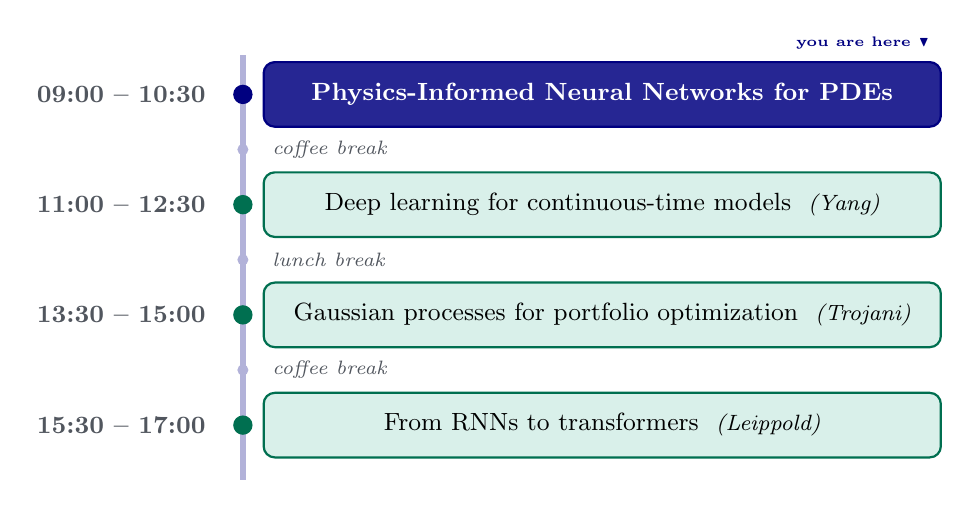
\begin{tikzpicture}[
    session/.style={rectangle, rounded corners=4pt, draw=uzhblue, thick, fill=softblue!15,
                    minimum width=8.6cm, minimum height=0.82cm, align=left, font=\small,
                    inner xsep=10pt, anchor=west},
    now/.style={session, fill=uzhblue!85, draw=uzhblue, text=white, font=\small\bfseries},
    guest/.style={session, fill=softgreen!15, draw=softgreen!70!black},
    pause/.style={font=\scriptsize\itshape, text=uzhgreydark, anchor=west},
    time/.style={font=\small\bfseries, text=uzhgreydark, anchor=east}
]
    \draw[uzhblue!30, line width=2pt] (0,0.5) -- (0,-4.9);

    \node[time] at (-0.35, 0) {09:00 -- 10:30};
    \node[now]  at (0.25, 0) {Physics-Informed Neural Networks for PDEs};
    \fill[uzhblue] (0,0) circle (3.5pt);
    \node[font=\tiny\bfseries, text=uzhblue, anchor=south east] at (8.85,0.45) {you are here $\blacktriangledown$};

    \node[pause] at (0.25,-0.7) {coffee break};
    \fill[uzhblue!30] (0,-0.7) circle (2pt);

    \node[time] at (-0.35,-1.4) {11:00 -- 12:30};
    \node[guest] at (0.25,-1.4) {Deep learning for continuous-time models~~{\footnotesize\itshape (Yang)}};
    \fill[softgreen!70!black] (0,-1.4) circle (3.5pt);

    \node[pause] at (0.25,-2.1) {lunch break};
    \fill[uzhblue!30] (0,-2.1) circle (2pt);

    \node[time] at (-0.35,-2.8) {13:30 -- 15:00};
    \node[guest] at (0.25,-2.8) {Gaussian processes for portfolio optimization~~{\footnotesize\itshape (Trojani)}};
    \fill[softgreen!70!black] (0,-2.8) circle (3.5pt);

    \node[pause] at (0.25,-3.5) {coffee break};
    \fill[uzhblue!30] (0,-3.5) circle (2pt);

    \node[time] at (-0.35,-4.2) {15:30 -- 17:00};
    \node[guest] at (0.25,-4.2) {From RNNs to transformers~~{\footnotesize\itshape (Leippold)}};
    \fill[softgreen!70!black] (0,-4.2) circle (3.5pt);
\end{tikzpicture}
\end{center}

\vspace{0.1cm}
\begin{center}
{\footnotesize \textbf{Materials:}~\href{https://github.com/sischei/summer-school-AI-for-economics-and-finance-2026}{github.com/sischei/summer-school-AI-\ldots-2026}~~$\cdot$~~\textbf{Cloud:}~\href{https://nuvolos.cloud}{nuvolos.cloud}}
\end{center}
\end{frame}

% --- Slide 3: Outline ---
\begin{frame}{Outline}
\begin{enumerate}
    \item \textbf{From DEQNs to PINNs}\\
    {\small Bridging discrete and continuous time; the PINN loss.}

    \vspace{0.4em}
    \item \textbf{PINN Fundamentals}\\
    {\small Automatic differentiation for PDEs, collocation, training loop.}

    \vspace{0.4em}
    \item \textbf{Soft vs.\ Hard Boundary Conditions}\\
    {\small Trial solutions, 2D Poisson, practical guidance.}

    \vspace{0.4em}
    \item \textbf{Economic Applications: HJB Equation}\\
    {\small Cake-eating problem, scaled trial solution + hard BCs, Adam $\to$ L-BFGS, analytical benchmark; DGM as optional high-D architecture.}

    \vspace{0.4em}
    \item \textbf{Financial Applications: Black--Scholes}\\
    {\small Option pricing via PINNs, comparison with analytical formula.}

    \vspace{0.4em}
    \item \textbf{When to Use One, and What Goes Wrong}\\
    {\small PINNs vs.\ grid solvers, inverse problems, failure modes, and which notebooks to run.}
\end{enumerate}
\end{frame}

% --- Slide 4: Roadmap ---
\begin{frame}{Roadmap of This Lecture (90 min)}
\begin{columns}[T]
\column{0.48\textwidth}
\textbf{I.\ From DEQNs to PINNs}~~\mbox{\small (11 min)}
\begin{itemize}\setlength\itemsep{1pt}
    \item Discrete vs.\ continuous time, the PINN loss
    \item Finger exercise
\end{itemize}

\vspace{0.4em}
\textbf{II.\ PINN fundamentals}~~\mbox{\small (20 min)}
\begin{itemize}\setlength\itemsep{1pt}
    \item Autograd for PDEs, collocation, training loop
    \item Adam $\to$ L-BFGS in FP64; warm-up 1D ODE
\end{itemize}

\vspace{0.4em}
\textbf{III.\ Boundary conditions}~~\mbox{\small (17 min)}
\begin{itemize}\setlength\itemsep{1pt}
    \item Soft penalties vs.\ hard trial solutions
    \item 2D Poisson; finger exercise
\end{itemize}

\column{0.48\textwidth}
\textbf{IV.\ HJB equations}~~\mbox{\small (18 min)}
\begin{itemize}\setlength\itemsep{1pt}
    \item Cake-eating, scaled trial solution, hard BCs
    \item DGM as an optional high-dimensional architecture
\end{itemize}

\vspace{0.4em}
\textbf{V.\ Finance: Black--Scholes}~~\mbox{\small (8 min)}
\begin{itemize}\setlength\itemsep{1pt}
    \item Option pricing against the closed form
\end{itemize}

\vspace{0.4em}
\textbf{VI.\ When to use one}~~\mbox{\small (16 min)}
\begin{itemize}\setlength\itemsep{1pt}
    \item PINNs vs.\ grid solvers; inverse problems
    \item Failure modes; what to run
\end{itemize}
\end{columns}
\end{frame}

% ============================================================================
% PART I: FROM DEQNs TO PINNs
% ============================================================================

% --- Slide 4: Section Divider ---
\section{From DEQNs to PINNs}

\begin{frame}{}
\vfill
\begin{center}
{\Huge \textcolor{uzhblue}{\textbf{Part I}}}\\[12pt]
{\LARGE From DEQNs to PINNs}
\end{center}
\vfill
\end{frame}

% --- Slide 5: Recall the DEQN Loss ---
\begin{frame}{Recall: The DEQN Loss from Day 1}
\textbf{Yesterday morning} (\texttt{02\_DEQN.pdf}) \textbf{we trained} a neural network $\mathcal{N}_\theta$ to satisfy
economic equilibrium conditions in \emphc{discrete time}:
\[
\boxed{
\ell_\theta^{\text{DEQN}} = \frac{1}{N}\sum_{i=1}^{N}
\bigl\|G\bigl(\x_i,\,\mathcal{N}_\theta(\x_i)\bigr)\bigr\|^2
}
\]

\vspace{0.3em}
\begin{itemize}
    \item $G(\cdot) = 0$: Euler equations, budget constraints, market clearing
    \item Training points $\x_i$: simulated from the model's own dynamics
    \item \emphc{No labeled data needed}, structural equations \emph{are} the loss
\end{itemize}

\vspace{0.5em}
\textbf{Today's question:}
What if the economic model is formulated in \emphc{continuous time}?
\end{frame}

% --- Slide 6: Discrete vs Continuous Time ---
\begin{frame}{Discrete vs.\ Continuous Time}
\begin{columns}[T]
\column{0.47\textwidth}
\begin{block}{Discrete Time (DEQN)}
\centering\small
\vspace{0.2em}
Euler equation:\\[4pt]
$u'(c_t) = \beta\,\E{u'(c_{t+1})\,R_{t+1}}$\\[8pt]
State transition:\\[4pt]
$\x_{t+1} = h(\x_t, p(\x_t), \varepsilon_{t+1})$\\[8pt]
Loss: algebraic residual $G(\cdot) = 0$
\vspace{0.2em}
\end{block}

\column{0.47\textwidth}
\begin{exampleblock}{Continuous Time (PINN)}
\centering\small
\vspace{0.2em}
State evolution:\\[4pt]
$\mathrm{d}a = (ra - c)\,\mathrm{d}t + \sigma\,\mathrm{d}W$\\[8pt]
HJB equation:\\[4pt]
$\rho V = \max_c \bigl\{u(c) + V_a(ra-c) + \tfrac{1}{2}\sigma^2 V_{aa}\bigr\}$\\[8pt]
Loss: PDE residual $\mathcal{R}(\cdot) = 0$
\vspace{0.2em}
\end{exampleblock}
\end{columns}

\vspace{0.6em}
\begin{center}
{\small \emphc{Key shift:} from algebraic residuals to \textbf{differential} residuals, we need \emphc{derivatives} of the neural network. The diffusion term $\tfrac{1}{2}\sigma^2 V_{aa}$ is why \emphc{second} derivatives matter.}
\end{center}
\end{frame}

% --- Slide 7: Why Continuous Time? ---
\begin{frame}{Why Continuous Time Matters}
\textbf{Many frontier models} are formulated in continuous time:

\vspace{0.3em}
\begin{itemize}
    \item \emphc{Heterogeneous-agent models:} Achdou, Han, Lasry, Lions \& Moll (2022), income and wealth distribution dynamics via HJB--KFE systems

    \vspace{0.2em}
    \item \emphc{Mean-field games:} optimal policy with a continuum of interacting agents

    \vspace{0.2em}
    \item \emphc{Asset pricing:} Black--Scholes, Heston, jump-diffusion models

    \vspace{0.2em}
    \item \emphc{Macro-finance:} Brunnermeier \& Sannikov (2014), He \& Krishnamurthy (2013)
\end{itemize}

\vspace{0.4em}
\begin{block}{Where this sits in the summer school}
Day 1 solved equilibrium conditions in \emphc{discrete} time with DEQNs. This morning we do the \emphc{continuous-time} counterpart, and at 11:00 Yang takes the same machinery to heterogeneous-agent models, where the HJB is coupled to a Kolmogorov forward equation.
\end{block}
\end{frame}

% --- Slide 8: The PINN Loss ---
\begin{frame}{The PINN Loss Function}
\textbf{Core idea} (Raissi, Perdikaris \& Karniadakis, 2019):

\vspace{0.15em}
Given a PDE $\mathcal{D}[u](\x) = 0$ on domain $\Omega$ with boundary conditions
$\mathcal{B}[u](\x) = 0$ on $\partial\Omega$, define:

\vspace{0.1em}
\[
\boxed{
\ell_\theta^{\mathrm{PINN}} =
\underbrace{\frac{1}{N_r}\sum_{i=1}^{N_r}
\bigl|\mathcal{D}[\mathcal{N}_\theta](\x_i^r)\bigr|^2}_{\text{PDE residual}}
\;+\;
\underbrace{\frac{\lambda}{N_b}\sum_{j=1}^{N_b}
\bigl|\mathcal{B}[\mathcal{N}_\theta](\x_j^b)\bigr|^2}_{\text{boundary/initial conditions}}
}
\]

\vspace{0.05em}
\begin{itemize}
    \item $\mathcal{N}_\theta$: neural network with parameters $\theta$
    \item $\x_i^r$: \emphc{collocation points} in the interior of $\Omega$
    \item $\x_j^b$: points on the boundary $\partial\Omega$
    \item Derivatives $\mathcal{D}[\mathcal{N}_\theta]$ computed via \emphc{automatic differentiation}
\end{itemize}
{\scriptsize \textbf{Warm-up ODE:} for $u''(x)=-1$ on $(0,1)$ with $u(0)=u(1)=0$, use $\mathcal{D}[u]=u''+1$ in the interior and $\mathcal{B}[u]=(u(0),u(1))$ on the boundary.}
\end{frame}

% --- Finger Exercise: PINN Loss ---
\begin{frame}{\exercisepause{} Finger Exercise: Writing a PINN Loss}
\begin{exampleblock}{Exercise (5 min)}
Consider the ODE $u''(x) = -1$ on $[0,1]$ with boundary conditions $u(0) = u(1) = 0$.
\begin{enumerate}
    \item Write down the PINN residual $\mathcal{R}(x; \theta) = \ldots$ using a neural network $\mathcal{N}(x; \theta)$.
    \item Write the total PINN loss as a sum of a PDE residual term and a boundary term.
    \item What is the exact solution?
\end{enumerate}
\end{exampleblock}
\end{frame}

\begin{frame}{Solution: Writing a PINN Loss}
\begin{block}{Answer}
\begin{enumerate}
    \item $\mathcal{R}(x; \theta) = \frac{\partial^2 \mathcal{N}}{\partial x^2}(x; \theta) + 1$.
    \item $\mathcal{L}(\theta) = \underbrace{\frac{1}{N_r}\sum_{i=1}^{N_r} \bigl|\mathcal{R}(x_i; \theta)\bigr|^2}_{\text{PDE residual}} + \lambda\,\underbrace{\bigl[\mathcal{N}(0;\theta)^2 + \mathcal{N}(1;\theta)^2\bigr]}_{\text{boundary conditions}}$
    \item $u(x) = \tfrac{1}{2}x(1-x)$ satisfies $u''=-1$, $u(0)=u(1)=0$. \checkmark
\end{enumerate}
\end{block}
\end{frame}

% --- Slide 9: DEQN vs PINN Side-by-Side ---
\begin{frame}{DEQN vs.\ PINN: Side-by-Side}
\begin{center}
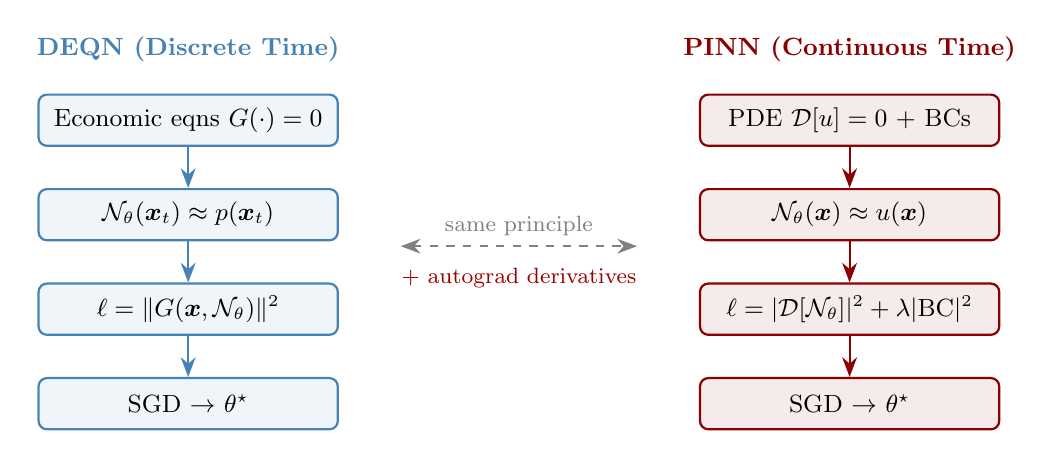
\begin{tikzpicture}[
    deqnbox/.style={rectangle, draw=softblue, thick, fill=softblue!8,
        minimum width=3.8cm, minimum height=0.65cm, font=\small,
        rounded corners=3pt},
    pinnbox/.style={rectangle, draw=darkred, thick, fill=darkred!8,
        minimum width=3.8cm, minimum height=0.65cm, font=\small,
        rounded corners=3pt},
    deqnarr/.style={-{Stealth[length=2.5mm]}, thick, softblue},
    pinnarr/.style={-{Stealth[length=2.5mm]}, thick, darkred}
]
    % DEQN column
    \node[font=\small\bfseries, softblue] at (-4.2,3.5) {DEQN (Discrete Time)};
    \node[deqnbox] (d1) at (-4.2,2.6) {Economic eqns $G(\cdot)=0$};
    \node[deqnbox] (d2) at (-4.2,1.4) {$\mathcal{N}_\theta(\x_t) \approx p(\x_t)$};
    \node[deqnbox] (d3) at (-4.2,0.2) {$\ell = \|G(\x, \mathcal{N}_\theta)\|^2$};
    \node[deqnbox] (d4) at (-4.2,-1.0) {SGD $\to$ $\theta^\star$};
    \draw[deqnarr] (d1) -- (d2);
    \draw[deqnarr] (d2) -- (d3);
    \draw[deqnarr] (d3) -- (d4);

    % PINN column
    \node[font=\small\bfseries, darkred] at (4.2,3.5) {PINN (Continuous Time)};
    \node[pinnbox] (p1) at (4.2,2.6) {PDE $\mathcal{D}[u]=0$ + BCs};
    \node[pinnbox] (p2) at (4.2,1.4) {$\mathcal{N}_\theta(\x) \approx u(\x)$};
    \node[pinnbox] (p3) at (4.2,0.2) {$\ell = |\mathcal{D}[\mathcal{N}_\theta]|^2 + \lambda|\text{BC}|^2$};
    \node[pinnbox] (p4) at (4.2,-1.0) {SGD $\to$ $\theta^\star$};
    \draw[pinnarr] (p1) -- (p2);
    \draw[pinnarr] (p2) -- (p3);
    \draw[pinnarr] (p3) -- (p4);

    % Arrow between
    \draw[dashed, thick, gray, {Stealth[length=2.5mm]}-{Stealth[length=2.5mm]}]
        (-1.5,1.0) -- (1.5,1.0)
        node[midway, above, font=\footnotesize, text=gray] {same principle};
    \node[below, font=\footnotesize, text=gray] at (0,0.85)
        {\emphc{+ autograd derivatives}};
\end{tikzpicture}
\end{center}

\vspace{0.3em}
{\small Both approaches are \emphc{unsupervised}: the physics (economics) \emph{is} the loss function.
The key addition for PINNs: we differentiate the network via any auto-diff tool (e.g.\ \texttt{torch.autograd.grad}).}
\end{frame}

% ============================================================================
% PART II: PINN FUNDAMENTALS
% ============================================================================

% --- Slide 10: Section Divider ---
\section{PINN Fundamentals}

\begin{frame}{}
\vfill
\begin{center}
{\Huge \textcolor{uzhblue}{\textbf{Part II}}}\\[12pt]
{\LARGE PINN Fundamentals}
\end{center}
\vfill
\end{frame}

% --- Slide 11: Automatic Differentiation ---
\begin{frame}[fragile]{Automatic Differentiation for PDEs}
\textbf{Key tool:} \texttt{torch.autograd.grad} with \texttt{create\_graph=True}.

\vspace{0.4em}
\begin{lstlisting}
# First derivative dy/dx
dydx = torch.autograd.grad(
    y, x,
    grad_outputs=torch.ones_like(y),
    create_graph=True   # keep graph for higher derivs
)[0]
\end{lstlisting}

\vspace{0.3em}
\begin{itemize}
    \item \texttt{create\_graph=True}: retains the computational graph so we can differentiate \emphc{again}
    \item This gives us \emphc{algorithmic} derivatives (up to floating-point precision), no finite differences!
    \item Works for \emphc{any order}: $\frac{\partial^n}{\partial x^n}$ by chaining $n$ calls
\end{itemize}
\end{frame}

% --- Slide 12: Second Derivatives ---
\begin{frame}[fragile]{Computing Second Derivatives}
\textbf{Chain two autograd calls} to get $y''(x)$:

\vspace{0.3em}
\begin{lstlisting}
# First derivative
dydx = torch.autograd.grad(
    y, x, grad_outputs=torch.ones_like(y),
    create_graph=True)[0]

# Second derivative
d2ydx2 = torch.autograd.grad(
    dydx, x, grad_outputs=torch.ones_like(dydx),
    create_graph=True)[0]
\end{lstlisting}

\vspace{0.3em}
\begin{center}
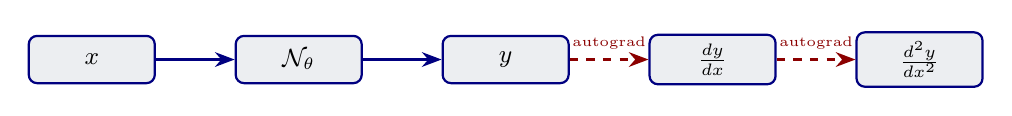
\begin{tikzpicture}[
    mlstep/.style={rectangle, draw=uzhblue, thick, fill=uzhgreylight,
        minimum width=1.6cm, minimum height=0.6cm, font=\small,
        rounded corners=3pt},
    arr/.style={-{Stealth[length=2.5mm]}, thick, uzhblue}
]
    \node[mlstep] (x) {$x$};
    \node[mlstep, right=1.0cm of x] (nn) {$\mathcal{N}_\theta$};
    \node[mlstep, right=1.0cm of nn] (y) {$y$};
    \node[mlstep, right=1.0cm of y] (dy) {$\frac{dy}{dx}$};
    \node[mlstep, right=1.0cm of dy] (d2y) {$\frac{d^2y}{dx^2}$};

    \draw[arr] (x) -- (nn);
    \draw[arr] (nn) -- (y);
    \draw[arr, dashed, darkred] (y) -- (dy) node[midway, above, font=\tiny] {autograd};
    \draw[arr, dashed, darkred] (dy) -- (d2y) node[midway, above, font=\tiny] {autograd};
\end{tikzpicture}
\end{center}
\end{frame}

% --- Slide 13: Collocation Points ---
\begin{frame}[fragile]{Collocation Points}
PINNs evaluate the PDE residual at \emphc{randomly sampled} points, no grid required.

\vspace{0.3em}
\begin{center}
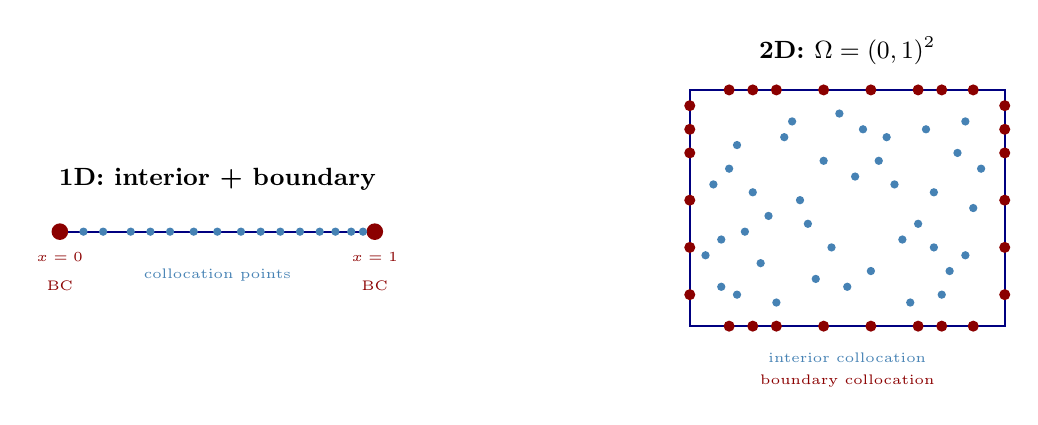
\begin{tikzpicture}
% 1D
\begin{scope}[shift={(-4.5,0)}]
    \draw[thick, uzhblue] (0,0) -- (4,0);
    \fill[darkred] (0,0) circle (3pt) node[below=4pt, font=\tiny] {$x=0$};
    \fill[darkred] (4,0) circle (3pt) node[below=4pt, font=\tiny] {$x=1$};
    \foreach \rx in {0.3,0.55,0.9,1.15,1.4,1.7,2.0,2.3,2.55,2.8,3.05,3.3,3.5,3.7,3.85}{
        \fill[softblue] (\rx,0) circle (1.5pt);
    }
    \node[above, font=\small\bfseries] at (2,0.4) {1D: interior + boundary};
    \node[below=10pt, font=\tiny, softblue] at (2,0) {collocation points};
    \node[below=10pt, font=\tiny, darkred] at (0,-0.15) {BC};
    \node[below=10pt, font=\tiny, darkred] at (4,-0.15) {BC};
\end{scope}

% 2D
\begin{scope}[shift={(3.5,-1.2)}]
    \draw[thick, uzhblue] (0,0) rectangle (4,3);
    % interior points (deterministic pseudo-random)
    \foreach \pt in {
        {0.4,0.5},{1.1,0.3},{2.3,0.7},{3.2,0.4},{0.7,1.2},{1.8,1.0},
        {2.9,1.3},{3.5,0.9},{0.3,1.8},{1.4,1.6},{2.1,1.9},{3.1,1.7},
        {0.6,2.3},{1.7,2.1},{2.5,2.4},{3.4,2.2},{0.9,0.8},{1.3,2.6},
        {2.7,1.1},{3.6,1.5},{0.5,2.0},{1.0,1.4},{2.0,0.5},{3.0,2.5},
        {0.2,0.9},{1.6,0.6},{2.4,2.1},{3.3,0.7},{0.8,1.7},{2.6,1.8},
        {1.2,2.4},{3.7,2.0},{0.4,1.1},{1.9,2.7},{2.8,0.3},{3.5,2.6},
        {0.6,0.4},{1.5,1.3},{2.2,2.5},{3.1,1.0}}{
        \fill[softblue] (\pt) circle (1.5pt);
    }
    % boundary points
    \foreach \rt in {0.5,1.1,1.7,2.3,2.9,3.2,3.6,0.8}{
        \fill[darkred] (\rt,0) circle (2pt);
        \fill[darkred] (\rt,3) circle (2pt);
    }
    \foreach \rt in {0.4,1.0,1.6,2.2,2.5,2.8}{
        \fill[darkred] (0,\rt) circle (2pt);
        \fill[darkred] (4,\rt) circle (2pt);
    }
    \node[above, font=\small\bfseries] at (2,3.2) {2D: $\Omega = (0,1)^2$};
    \node[font=\tiny, softblue] at (2,-0.4) {interior collocation};
    \node[font=\tiny, darkred] at (2,-0.7) {boundary collocation};
\end{scope}
\end{tikzpicture}
\end{center}

\vspace{0.2em}
{\small Points are \emphc{resampled} periodically during training to avoid overfitting to a fixed set.}
\end{frame}

% --- Slide 14: PINN Training Algorithm ---
\begin{frame}{PINN Training Algorithm}
\begin{block}{Algorithm: Physics-Informed Neural Network Training}
\begin{algorithmic}
\footnotesize
\STATE \textbf{Input:} PDE $\mathcal{D}[u]=0$, BCs $\mathcal{B}[u]=0$, network $\mathcal{N}_\theta$, learning rate $\eta$
\FOR{epoch $= 1, \ldots, E$}
    \STATE Sample $N_r$ collocation points $\{\x_i^r\}$ in domain $\Omega$
    \STATE Sample $N_b$ boundary points $\{\x_j^b\}$ on $\partial\Omega$
    \STATE Forward pass: compute $\mathcal{N}_\theta(\x_i^r)$ and $\mathcal{N}_\theta(\x_j^b)$
    \STATE Autograd: compute $\mathcal{D}[\mathcal{N}_\theta](\x_i^r)$ via \texttt{torch.autograd.grad}
    \STATE $\ell_\theta = \frac{1}{N_r}\sum_i |\mathcal{D}[\mathcal{N}_\theta](\x_i^r)|^2 + \frac{\lambda}{N_b}\sum_j |\mathcal{B}[\mathcal{N}_\theta](\x_j^b)|^2$
    \STATE Update: $\theta \leftarrow \theta - \eta\,\nabla_\theta \ell_\theta$
\ENDFOR
\STATE \textbf{Output:} Trained $\mathcal{N}_{\theta^\star}$ approximating the PDE solution
\end{algorithmic}
\end{block}

\vspace{0.2em}
{\small \textbf{Note:} Unlike DEQNs, training points are \emphc{not} simulated from model dynamics, they are drawn uniformly (or adaptively) from the domain.}
\end{frame}

% --- Slide 14b: Optimizer pipeline and FP64 ---
\begin{frame}{Optimizer Pipeline: Adam $\to$ L-BFGS, in FP64}
\small
\begin{columns}[T]
\column{0.50\textwidth}
\textbf{Two stages.}
\begin{itemize}\itemsep0pt
    \item \emphc{Adam} on resampled collocation: finds a basin.
    \item \emphc{Deterministic L-BFGS} on a \emph{fixed} grid: closes the residual. Resampling per evaluation breaks the line search.
\end{itemize}

\vspace{0.3em}
\textbf{Why FP64?}
\begin{itemize}\itemsep0pt
    \item $\tanh$-MLP second derivatives lose $\sim$7 digits in FP32.
    \item The Wolfe search compares values at exactly that scale.
    \item FP32 plateaus at the noise floor; FP64 keeps going.
\end{itemize}

\column{0.48\textwidth}
\begin{block}{Practical recipe}
\footnotesize
\textbf{1.}~Cast model + data to \texttt{float64}.\\
\textbf{2.}~Adam, lr $10^{-3}$, a few k epochs, resampled collocation.\\
\textbf{3.}~Freeze grid; \texttt{torch.optim.LBFGS} (strong-Wolfe).\\
\textbf{4.}~Stop on residual stagnation.
\end{block}
{\footnotesize Precision evidence: \href{https://arxiv.org/abs/2505.10949}{arXiv:2505.10949}.}
\end{columns}

\vspace{0.2em}
{\footnotesize \emphc{Used in notebooks 04 and 05.} Report PDE residuals and solution diagnostics, not the optimizer label.}
\end{frame}

% --- Slide 15: PINN Architecture ---
\begin{frame}{PINN Architecture}
\begin{center}
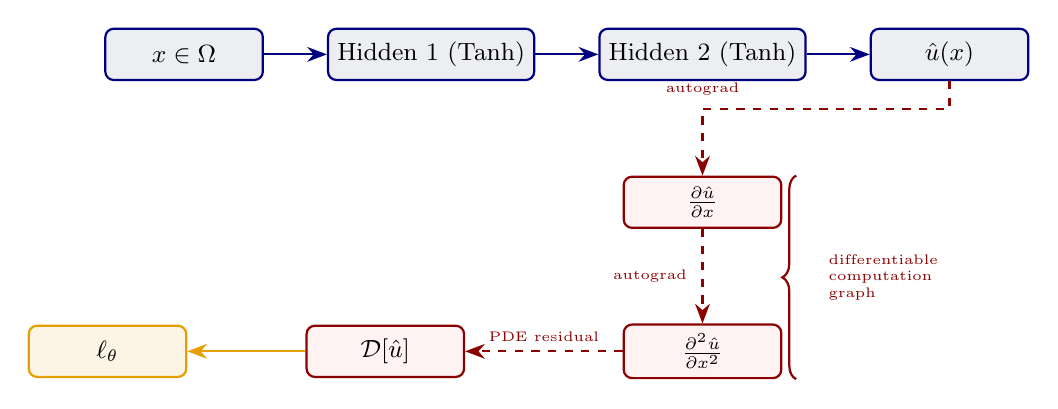
\begin{tikzpicture}[
    mlstep/.style={rectangle, draw=uzhblue, thick, fill=uzhgreylight,
        minimum width=2.0cm, minimum height=0.65cm, font=\small,
        rounded corners=3pt},
    deriv/.style={rectangle, draw=darkred, thick, fill=red!5,
        minimum width=2.0cm, minimum height=0.65cm, font=\small,
        rounded corners=3pt},
    arr/.style={-{Stealth[length=2.5mm]}, thick, uzhblue},
    darr/.style={-{Stealth[length=2.5mm]}, thick, dashed, darkred}
]
    % Main forward path
    \node[mlstep] (in) {$x \in \Omega$};
    \node[mlstep, right=0.8cm of in] (h1) {Hidden 1 (Tanh)};
    \node[mlstep, right=0.8cm of h1] (h2) {Hidden 2 (Tanh)};
    \node[mlstep, right=0.8cm of h2] (out) {$\hat{u}(x)$};

    \draw[arr] (in) -- (h1);
    \draw[arr] (h1) -- (h2);
    \draw[arr] (h2) -- (out);

    % Autograd branch --- shifted left, more vertical spacing
    \node[deriv, below=1.2cm of h2] (du) {$\frac{\partial \hat{u}}{\partial x}$};
    \node[deriv, below=1.2cm of du] (d2u) {$\frac{\partial^2 \hat{u}}{\partial x^2}$};

    \draw[darr] (out.south) -- ++(0,-0.35) -| (du.north)
        node[pos=0.5, above=1pt, font=\tiny] {autograd};
    \draw[darr] (du) -- (d2u) node[midway, left=2pt, font=\tiny] {autograd};

    % PDE residual and loss
    \node[deriv, left=2.0cm of d2u] (res) {$\mathcal{D}[\hat{u}]$};
    \node[rectangle, draw=softorange, thick, fill=softorange!10,
        minimum width=2.0cm, minimum height=0.65cm, font=\small,
        rounded corners=3pt, left=1.5cm of res] (loss) {$\ell_\theta$};

    \draw[darr] (d2u) -- (res) node[midway, above, font=\tiny] {PDE residual};
    \draw[-{Stealth[length=2.5mm]}, thick, softorange] (res) -- (loss);

    % Brace annotation
    \draw[decorate, decoration={brace, amplitude=5pt, mirror}, thick, darkred]
        ([xshift=5pt]du.north east) -- ([xshift=5pt]d2u.south east)
        node[midway, right=8pt, font=\tiny, text=darkred, align=left]
        {differentiable\\computation\\graph};
\end{tikzpicture}
\end{center}

\vspace{0.2em}
{\small The entire pipeline, forward pass \emph{and} derivative computation, is \emphc{differentiable}, enabling end-to-end gradient-based training.}
\end{frame}

% --- Slide 16: Why Tanh? ---
\begin{frame}{Why Tanh Activations for PINNs?}
\begin{columns}[T]
\column{0.55\textwidth}
\textbf{PDE residuals require smooth derivatives.}

\vspace{0.3em}
\begin{itemize}
    \item \emphc{ReLU}: $C^0$ only; its second derivative vanishes almost everywhere, so a $u''$ residual carries no gradient
    \item \emphc{Tanh}: $C^\infty$, all derivatives are well-defined and informative
    \item \emphc{Softplus}: $C^\infty$, useful for positivity constraints (e.g.\ consumption)
\end{itemize}

\vspace{0.5em}
\begin{alertblock}{Rule of thumb}
For PINNs requiring $k$-th order derivatives, use activations that are at least $C^k$.
\end{alertblock}

\column{0.42\textwidth}
\begin{center}
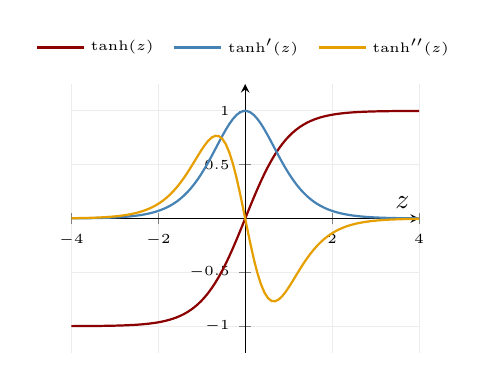
\begin{tikzpicture}
\begin{axis}[
    width=6cm, height=5cm,
    xlabel={$z$}, xlabel style={font=\small},
    tick label style={font=\tiny},
    xmin=-4, xmax=4, ymin=-1.25, ymax=1.25,
    ytick={-1,-0.5,0.5,1},
    grid=major, grid style={gray!15},
    axis lines=middle,
    legend columns=3,
    legend style={font=\tiny, draw=none, fill=none, at={(0.5,1.06)}, anchor=south,
                  /tikz/every even column/.append style={column sep=5pt}},
]
    \addplot[thick, darkred, domain=-4:4, samples=100]{tanh(x)};
    \addlegendentry{$\tanh(z)$}
    \addplot[thick, softblue, domain=-4:4, samples=100]{1 - tanh(x)^2};
    \addlegendentry{$\tanh'(z)$}
    \addplot[thick, softorange, domain=-4:4, samples=100]
        {-2*tanh(x)*(1 - tanh(x)^2)};
    \addlegendentry{$\tanh''(z)$}
\end{axis}
\end{tikzpicture}
\end{center}
\end{columns}
\end{frame}

% --- Slide 17: Warm-up ODE ---
\begin{frame}{Warm-up: Solving an ODE with a PINN}
\textbf{Problem:} $y''(x) = -1$ on $(0,1)$, \; $y(0) = y(1) = 0$.
\quad \textbf{Analytical:} $y(x) = \tfrac{1}{2}x(1-x)$.

\vspace{0.5em}
\begin{columns}[T]
\column{0.48\textwidth}
\textbf{PINN setup:}
\begin{enumerate}\setlength{\itemsep}{3pt}
    \item NN $\mathcal{N}_\theta : [0,1] \to \R$, 2 hidden layers of 20 units, $\tanh$
    \item Residual: $r(x) = \mathcal{N}_\theta''(x) + 1$
    \item Loss: PDE residual + BC penalty (soft, here)
\end{enumerate}

\vspace{0.5em}
\[
\ell = \frac{1}{N}\!\sum_i r(x_i)^2 + \mathcal{N}_\theta(0)^2 + \mathcal{N}_\theta(1)^2
\]

\column{0.50\textwidth}
\textbf{After 5{,}000 Adam epochs:}
\begin{itemize}\setlength\itemsep{3pt}
    \item Final loss $\approx 2\times10^{-5}$, of which the BC term is $\approx 9\times10^{-6}$
    \item Max absolute error $1.9\times10^{-3}$, mean $1.8\times10^{-3}$
\end{itemize}

\vspace{0.5em}
\begin{block}{Read the error, not the loss}
\footnotesize
A small loss says the residual is small at the sampled points. Only the comparison against $\tfrac12x(1-x)$ says the \emph{solution} is right.
\end{block}
\end{columns}

\vspace{0.4em}
{\small\hfill\textbf{Notebook:} \texttt{01\_ODE\_PINN\_ZeroBCs}}
\end{frame}

% --- Slide 17b: Warm-up result, full width so the axes are readable ---
\begin{frame}{Warm-up: PINN vs.\ Analytical Solution}
\begin{center}
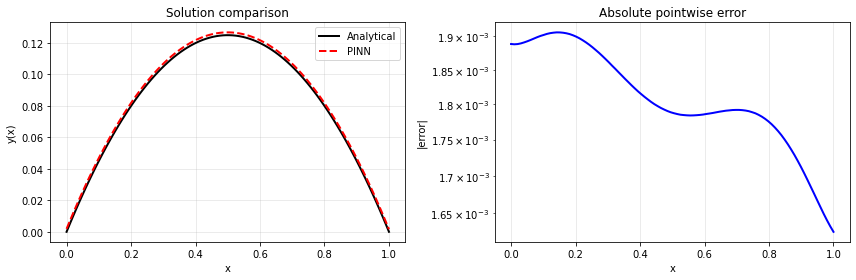
\includegraphics[width=\linewidth,keepaspectratio]{figures/pinn_ode_warmup.png}
\end{center}

\vspace{0.4em}
{\footnotesize Left: the network on top of $y(x)=\tfrac12x(1-x)$ --- indistinguishable at this
scale. Right: the absolute error, which is what actually tells you how well it did. Note the axis:
it stays in a narrow band around $1.8\times10^{-3}$ across the domain, with no drift to the boundaries.}

\vspace{-0.1em}
{\small\hfill\textbf{Notebook:} \texttt{01\_ODE\_PINN\_ZeroBCs}}
\end{frame}

% --- Slide 18: Non-Zero BCs ---
\begin{frame}{Non-Zero Boundary Conditions: The Challenge}
\textbf{Problem:} $y''(x) = -1$ on $(0,1)$ with $y(0) = 1$, $y(1) = 2$.

\vspace{0.2em}
\textbf{Analytical solution:} $y(x) = -\tfrac{1}{2}x^2 + \tfrac{3}{2}x + 1$.

\vspace{0.4em}
\textbf{Soft BC enforcement:}
\[
\ell = \frac{1}{N}\sum_i r(x_i)^2 + \lambda_0\bigl(\mathcal{N}_\theta(0) - 1\bigr)^2 + \lambda_1\bigl(\mathcal{N}_\theta(1) - 2\bigr)^2
\]

\vspace{0.3em}
\textbf{Issues with soft enforcement:}
\begin{itemize}
    \item BCs are only \emphc{approximately} satisfied
    \item Penalty weight $\lambda$ requires \emphc{tuning}: too small $\Rightarrow$ BC violated; too large $\Rightarrow$ PDE ignored
    \item Boundary errors can \emphc{propagate} into the interior
\end{itemize}

\vspace{0.3em}
$\Rightarrow$ \textbf{Motivates hard boundary enforcement} (Part III).
\end{frame}

% ============================================================================
% PART III: SOFT vs HARD BOUNDARY CONDITIONS
% ============================================================================

% --- Slide 19: Section Divider ---
\section{Soft vs.\ Hard Boundary Conditions}

\begin{frame}{}
\vfill
\begin{center}
{\Huge \textcolor{uzhblue}{\textbf{Part III}}}\\[12pt]
{\LARGE Soft vs.\ Hard Boundary Conditions}
\end{center}
\vfill
\end{frame}

% --- Slide 19b: What Are Boundary Conditions? ---
\begin{frame}{What Are Boundary Conditions?}
\begin{center}
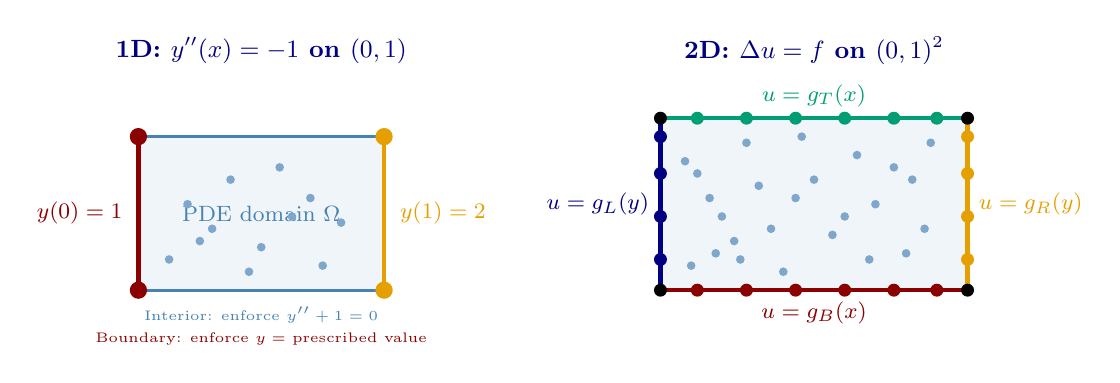
\begin{tikzpicture}[scale=0.78]
    % --- 1D example (left) ---
    \begin{scope}[shift={(-5.5,0)}]
        \node[font=\small\bfseries, uzhblue] at (2,3.9) {1D: $y''(x) = -1$ on $(0,1)$};

        % Domain line
        \draw[very thick, softblue, fill=softblue!8] (0,0) rectangle (4,2.5);
        \node[font=\footnotesize, softblue] at (2,1.25) {PDE domain $\Omega$};

        % Left boundary
        \draw[ultra thick, darkred] (0,0) -- (0,2.5);
        \node[left, font=\footnotesize, darkred] at (-0.1,1.25) {$y(0)=1$};
        \fill[darkred] (0,0) circle (4pt);
        \fill[darkred] (0,2.5) circle (4pt);

        % Right boundary
        \draw[ultra thick, softorange] (4,0) -- (4,2.5);
        \node[right, font=\footnotesize, softorange] at (4.1,1.25) {$y(1)=2$};
        \fill[softorange] (4,0) circle (4pt);
        \fill[softorange] (4,2.5) circle (4pt);

        % Interior collocation dots
        \foreach \pt in {{0.5,0.5},{1.2,1.0},{2.0,0.7},{2.8,1.5},{1.5,1.8},
            {3.0,0.4},{0.8,1.4},{2.3,2.0},{3.3,1.1},{1.0,0.8},{2.5,1.2},{1.8,0.3}}{
            \fill[softblue!70] (\pt) circle (2pt);
        }
        \node[font=\tiny, softblue] at (2,-0.4) {Interior: enforce $y''+1=0$};
        \node[font=\tiny, darkred] at (2,-0.8) {Boundary: enforce $y=$ prescribed value};
    \end{scope}

    % --- 2D example (right) ---
    \begin{scope}[shift={(3.0,0)}]
        \node[font=\small\bfseries, uzhblue] at (2.5,3.9) {2D: $\Delta u = f$ on $(0,1)^2$};

        % Domain
        \fill[softblue!8] (0,0) rectangle (5,2.8);

        % Boundary sides with different colors
        \draw[ultra thick, darkred] (0,0) -- (5,0)
            node[midway, below, font=\footnotesize] {$u = g_B(x)$};
        \draw[ultra thick, softorange] (5,0) -- (5,2.8)
            node[midway, right, font=\footnotesize] {$u = g_R(y)$};
        \draw[ultra thick, softgreen] (0,2.8) -- (5,2.8)
            node[midway, above, font=\footnotesize] {$u = g_T(x)$};
        \draw[ultra thick, uzhblue] (0,0) -- (0,2.8)
            node[midway, left, font=\footnotesize] {$u = g_L(y)$};

        % Interior points
        \foreach \pt in {{0.5,0.4},{1.2,0.8},{2.0,0.3},{3.0,1.2},{4.0,0.6},
            {0.8,1.5},{1.8,1.0},{2.5,1.8},{3.5,1.4},{4.3,1.0},
            {0.4,2.1},{1.4,2.4},{2.2,1.5},{3.2,2.2},{4.1,1.8},
            {0.9,0.6},{1.6,1.7},{2.8,0.9},{3.8,2.0},{1.0,1.2},
            {2.3,2.5},{3.4,0.5},{4.4,2.4},{0.6,1.9},{1.3,0.5}}{
            \fill[softblue!70] (\pt) circle (2pt);
        }

        % Boundary points
        \foreach \rt in {0.6,1.4,2.2,3.0,3.8,4.5}{
            \fill[darkred] (\rt,0) circle (3pt);
            \fill[softgreen] (\rt,2.8) circle (3pt);
        }
        \foreach \rt in {0.5,1.2,1.9,2.5}{
            \fill[uzhblue] (0,\rt) circle (3pt);
            \fill[softorange] (5,\rt) circle (3pt);
        }

        % Corner markers
        \fill[black] (0,0) circle (3pt);
        \fill[black] (5,0) circle (3pt);
        \fill[black] (0,2.8) circle (3pt);
        \fill[black] (5,2.8) circle (3pt);
    \end{scope}
\end{tikzpicture}
\end{center}

\vspace{0.2em}
\begin{block}{Two enforcement strategies}
\textbf{Soft:} add BC violation as a penalty term in the loss.\\
\textbf{Hard:} build BCs into the network output by construction.
\end{block}
\end{frame}

% --- Slide 19c: Visual: Soft BC Problems ---
\begin{frame}{The Problem with Soft Boundary Conditions}
\begin{center}
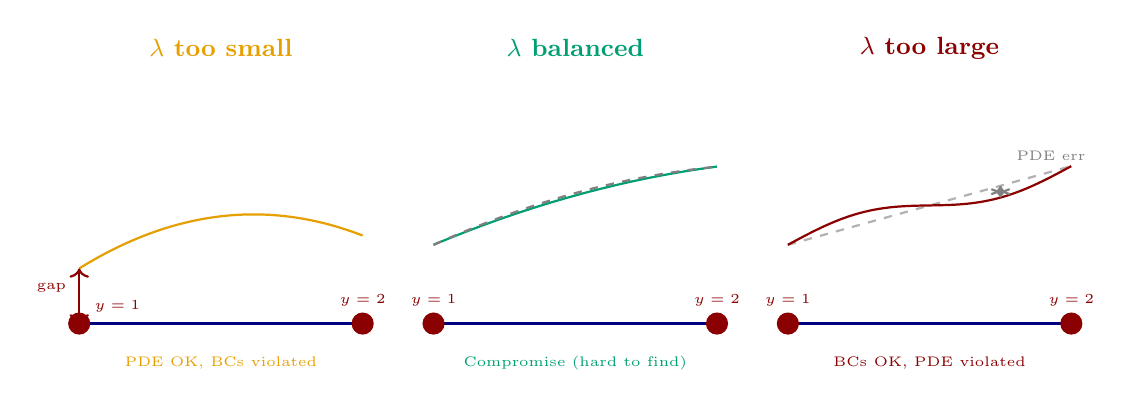
\begin{tikzpicture}
    % Three scenarios
    % Lambda too small
    \begin{scope}[shift={(-5,0)}]
        \node[font=\small\bfseries, softorange] at (1.8,3.5) {$\lambda$ too small};
        \draw[thick, uzhblue] (0,0) -- (3.6,0);
        \fill[darkred] (0,0) circle (4pt);
        \fill[darkred] (3.6,0) circle (4pt);
        \node[above right=-1pt and 2pt, font=\tiny, darkred] at (0,0.05) {$y=1$};
        \node[above, font=\tiny, darkred] at (3.6,0.1) {$y=2$};
        % Solution that misses BCs
        \draw[thick, softorange, domain=0:3.6, samples=60]
            plot (\x, {-0.14*\x*\x + 0.62*\x + 0.7});
        \node[font=\tiny, softorange] at (1.8,-0.5) {PDE OK, BCs violated};
        % Show BC mismatch
        \draw[thick, darkred, <->] (0,0) -- (0,0.7) node[pos=0.65, left=1pt, font=\tiny] {gap};
    \end{scope}

    % Lambda balanced
    \begin{scope}[shift={(-0.5,0)}]
        \node[font=\small\bfseries, softgreen] at (1.8,3.5) {$\lambda$ balanced};
        \draw[thick, uzhblue] (0,0) -- (3.6,0);
        \fill[darkred] (0,0) circle (4pt);
        \fill[darkred] (3.6,0) circle (4pt);
        \node[above, font=\tiny, darkred] at (0,0.1) {$y=1$};
        \node[above, font=\tiny, darkred] at (3.6,0.1) {$y=2$};
        % Good solution
        \draw[thick, softgreen, domain=0:3.6, samples=60]
            plot (\x, {-0.04*\x*\x + 0.42*\x + 1.0});
        % Analytical for reference (dashed)
        \draw[thick, dashed, gray, domain=0:3.6, samples=60]
            plot (\x, {-0.04*\x*\x + 0.42*\x + 1.0 + 0.03*sin(deg(3.14*\x/3.6))});
        \node[font=\tiny, softgreen] at (1.8,-0.5) {Compromise (hard to find)};
    \end{scope}

    % Lambda too large
    \begin{scope}[shift={(4,0)}]
        \node[font=\small\bfseries, darkred] at (1.8,3.5) {$\lambda$ too large};
        \draw[thick, uzhblue] (0,0) -- (3.6,0);
        \fill[darkred] (0,0) circle (4pt);
        \fill[darkred] (3.6,0) circle (4pt);
        \node[above, font=\tiny, darkred] at (0,0.1) {$y=1$};
        \node[above, font=\tiny, darkred] at (3.6,0.1) {$y=2$};
        % Reference straight interpolation (BC-consistent, PDE-consistent target)
        \draw[thick, dashed, gray!60] (0,1.0) -- (3.6,2.0);
        % Solution that nails BCs but bad interior
        \draw[thick, darkred, domain=0:3.6, samples=60]
            plot (\x, {1.0 + \x/3.6 + 0.15*sin(deg(2*3.14*\x/3.6))});
        \node[font=\tiny, darkred] at (1.8,-0.5) {BCs OK, PDE violated};
        % Show interior wiggle (deviation from reference at x=2.7, the trough)
        \draw[thick, gray, <->] (2.7,1.6) -- (2.7,1.75);
        \node[font=\tiny, gray, anchor=south west] at (2.78,1.95) {PDE err};
    \end{scope}
\end{tikzpicture}
\end{center}

\vspace{0.4em}
\begin{center}
{\small Soft BCs require \emphc{careful balancing} of the penalty weight $\lambda$.\\
Too small: BCs violated. Too large: PDE ignored. Just right: hard to find \emph{a priori}.}
\end{center}
\end{frame}

% --- Slide 20: Hard BC Trial Solution ---
\begin{frame}{Hard BC Enforcement: Trial Solutions}
\textbf{Idea:} construct a \emphc{trial solution} that satisfies BCs \emph{by construction}:
\[
\boxed{
\hat{y}(x) = A(x) + B(x)\cdot\mathcal{N}_\theta(x)
}
\]

\vspace{0.2em}
where:
\begin{itemize}
    \item $A(x)$: \emphc{anchor function} satisfying the BCs exactly, e.g.\ $A(x) = 1 + x$
    \item $B(x)$: \emphc{mask function} vanishing at boundaries, e.g.\ $B(x) = x(1-x)$
    \item $\mathcal{N}_\theta(x)$: free neural network (no BC constraints)
\end{itemize}

\vspace{0.3em}
\textbf{Verification:}
\begin{align*}
\hat{y}(0) &= A(0) + B(0)\cdot\mathcal{N}_\theta(0) = 1 + 0 = 1 \quad\checkmark\\
\hat{y}(1) &= A(1) + B(1)\cdot\mathcal{N}_\theta(1) = 2 + 0 = 2 \quad\checkmark
\end{align*}

$\Rightarrow$ BCs hold \emphc{identically}, only the PDE residual loss remains.
\end{frame}

% --- Slide 20b: Trial Solution Visual Decomposition ---
\begin{frame}{Trial Solution: Visual Decomposition}
\vspace{-0.3em}
\begin{center}
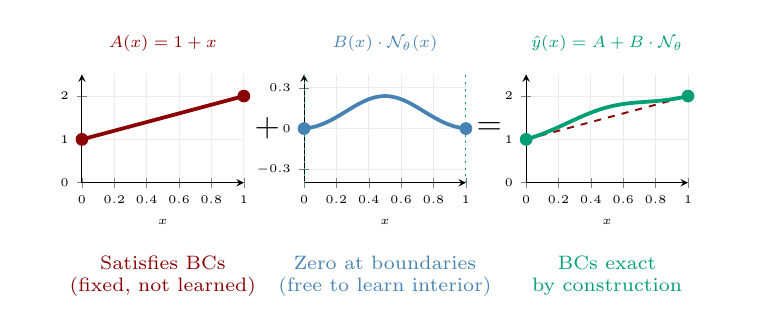
\begin{tikzpicture}[scale=0.85]
    % A(x) plot
    \begin{axis}[
        name=plotA,
        width=4.0cm, height=3.2cm,
        title={\scriptsize $A(x) = 1 + x$},
        title style={font=\scriptsize\bfseries, text=darkred},
        xlabel={$x$}, xlabel style={font=\tiny},
        ylabel style={font=\tiny},
        tick label style={font=\tiny},
        xmin=0, xmax=1, ymin=0, ymax=2.5,
        grid=major, grid style={gray!15},
        axis lines=left,
    ]
        \addplot[ultra thick, darkred, domain=0:1, samples=2]{1+x};
        \addplot[only marks, mark=*, mark size=2.5pt, darkred]
            coordinates {(0,1) (1,2)};
    \end{axis}

    % Plus sign
    \node[font=\large\bfseries] at ($(plotA.east)+(0.35,0)$) {$+$};

    % B(x) * N(x) plot
    \begin{axis}[
        at={($(plotA.east)+(0.9cm,0)$)}, anchor=west,
        name=plotBN,
        width=4.0cm, height=3.2cm,
        title={\scriptsize $B(x)\cdot\mathcal{N}_\theta(x)$},
        title style={font=\scriptsize\bfseries, text=softblue},
        xlabel={$x$}, xlabel style={font=\tiny},
        ylabel style={font=\tiny},
        tick label style={font=\tiny},
        xmin=0, xmax=1, ymin=-0.4, ymax=0.4,
        ytick={-0.3,0,0.3},
        grid=major, grid style={gray!15},
        axis lines=left,
    ]
        \addplot[ultra thick, softblue, domain=0:1, samples=80]
            {0.6*x*(1-x)*(0.8*sin(deg(3.14*x)) - 0.3*cos(deg(2*3.14*x)) + 0.5)};
        \addplot[only marks, mark=*, mark size=2.5pt, softblue]
            coordinates {(0,0) (1,0)};
        \draw[thick, softgreen, dotted] (axis cs:0,-0.4) -- (axis cs:0,0.4);
        \draw[thick, softgreen, dotted] (axis cs:1,-0.4) -- (axis cs:1,0.4);
    \end{axis}

    % Equals sign
    \node[font=\large\bfseries] at ($(plotBN.east)+(0.35,0)$) {$=$};

    % y_hat(x) plot
    \begin{axis}[
        at={($(plotBN.east)+(0.9cm,0)$)}, anchor=west,
        name=plotY,
        width=4.0cm, height=3.2cm,
        title={\scriptsize $\hat{y}(x) = A + B\cdot\mathcal{N}_\theta$},
        title style={font=\scriptsize\bfseries, text=softgreen},
        xlabel={$x$}, xlabel style={font=\tiny},
        ylabel style={font=\tiny},
        tick label style={font=\tiny},
        xmin=0, xmax=1, ymin=0, ymax=2.5,
        grid=major, grid style={gray!15},
        axis lines=left,
    ]
        \addplot[thick, dashed, darkred, domain=0:1, samples=2]{1+x};
        \addplot[ultra thick, softgreen, domain=0:1, samples=80]
            {1 + x + 0.6*x*(1-x)*(0.8*sin(deg(3.14*x)) - 0.3*cos(deg(2*3.14*x)) + 0.5)};
        \addplot[only marks, mark=*, mark size=2.5pt, softgreen]
            coordinates {(0,1) (1,2)};
    \end{axis}

    % Annotations below the x-axis labels, constrained to plot width so they
    % don't bleed into neighboring plots
    \node[font=\scriptsize, darkred, align=center, anchor=north,
          text width=3.2cm] at ($(plotA.south)-(0,0.95)$)
        {Satisfies BCs\\(fixed, not learned)};
    \node[font=\scriptsize, softblue, align=center, anchor=north,
          text width=3.2cm] at ($(plotBN.south)-(0,0.95)$)
        {Zero at boundaries\\(free to learn interior)};
    \node[font=\scriptsize, softgreen, align=center, anchor=north,
          text width=3.2cm] at ($(plotY.south)-(0,0.95)$)
        {BCs exact\\by construction};
\end{tikzpicture}
\end{center}
\end{frame}

% --- Slide 21: Hard BC Code ---
\begin{frame}[fragile]{Hard BC: Implementation}
\begin{lstlisting}[basicstyle=\scriptsize\ttfamily]
def A(x):                          # Anchor: A(0)=1, A(1)=2
    return 1.0 + x
def B(x):                          # Mask: B(0)=B(1)=0
    return x * (1.0 - x)

def y_trial(model, x):            # Hard-BC trial solution
    return A(x) + B(x) * model(x)

def residual(model, x):
    x.requires_grad_(True)
    y = y_trial(model, x)
    dydx   = torch.autograd.grad(y, x, (*@\ldots@*))[0]
    d2ydx2 = torch.autograd.grad(dydx, x, (*@\ldots@*))[0]
    return d2ydx2 + 1.0           # should be 0
\end{lstlisting}

\vspace{0.2em}
{\small \textbf{Advantage:} the loss has \emphc{only one term} (PDE residual), no $\lambda$ to tune!}
\end{frame}

% --- Slide 21b: Visual: 2D Hard BC Construction ---
\begin{frame}{Hard BCs in 2D: Building the Trial Solution}
\begin{center}
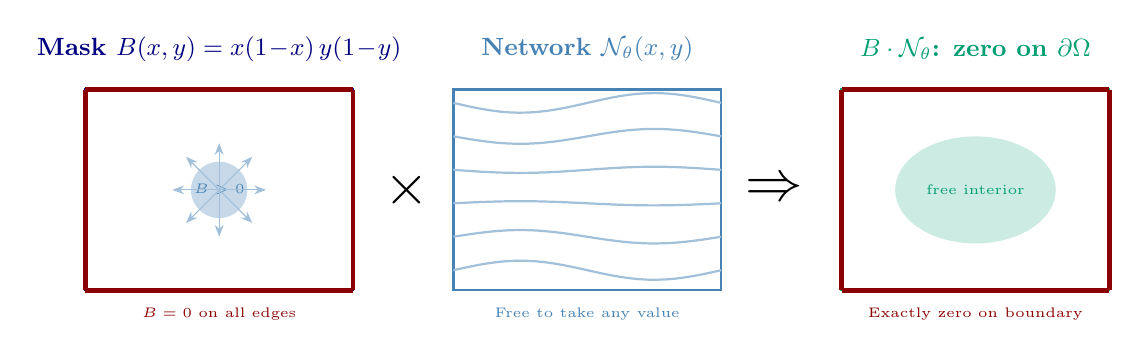
\begin{tikzpicture}[scale=0.85]
    % --- Mask B(x,y) ---
    \begin{scope}[shift={(-5.5,0)}]
        \node[font=\small\bfseries, uzhblue] at (2,3.6) {Mask $B(x,y) = x(1\!-\!x)\,y(1\!-\!y)$};
        % Domain square
        \draw[thick, uzhblue] (0,0) rectangle (4,3);
        % Zero on boundary (thick red)
        \draw[ultra thick, darkred] (0,0) -- (4,0);
        \draw[ultra thick, darkred] (4,0) -- (4,3);
        \draw[ultra thick, darkred] (4,3) -- (0,3);
        \draw[ultra thick, darkred] (0,3) -- (0,0);
        \node[font=\tiny, darkred] at (2,-0.35) {$B = 0$ on all edges};
        % Interior peak
        \fill[softblue!30] (2,1.5) circle (12pt);
        \node[font=\tiny, softblue] at (2,1.5) {$B > 0$};
        % Arrows showing B vanishes
        \foreach \a in {0,45,...,315}{
            \draw[-{Stealth[length=1.5mm]}, thin, softblue!50]
                (2,1.5) -- +(\a:0.7);
        }
    \end{scope}

    % Plus sign
    \node[font=\huge\bfseries] at (-0.7,1.5) {$\times$};

    % --- Network N(x,y) ---
    \begin{scope}[shift={(0,0)}]
        \node[font=\small\bfseries, softblue] at (2,3.6) {Network $\mathcal{N}_\theta(x,y)$};
        \draw[thick, softblue] (0,0) rectangle (4,3);
        % Wavy surface (NN output)
        \foreach \y in {0.3,0.8,...,2.8}{
            \draw[softblue!50, thick, domain=0:4, samples=30]
                plot (\x, {\y + 0.15*sin(deg(2*3.14*\x/4))*cos(deg(3.14*\y/3))});
        }
        \node[font=\tiny, softblue] at (2,-0.35) {Free to take any value};
    \end{scope}

    % Arrow to result
    \node[font=\huge\bfseries] at (4.8,1.5) {$\Rightarrow$};

    % --- Result B*N ---
    \begin{scope}[shift={(5.8,0)}]
        \node[font=\small\bfseries, softgreen] at (2,3.6) {$B \cdot \mathcal{N}_\theta$: zero on $\partial\Omega$};
        \draw[thick, softgreen] (0,0) rectangle (4,3);
        % Zero boundary (flat edges)
        \draw[ultra thick, darkred] (0,0) -- (4,0);
        \draw[ultra thick, darkred] (4,0) -- (4,3);
        \draw[ultra thick, darkred] (4,3) -- (0,3);
        \draw[ultra thick, darkred] (0,3) -- (0,0);
        % Interior variation (damped by B)
        \fill[softgreen!20] (2,1.5) ellipse (1.2 and 0.8);
        \node[font=\tiny, softgreen] at (2,1.5) {free interior};
        \node[font=\tiny, darkred] at (2,-0.35) {Exactly zero on boundary};
    \end{scope}
\end{tikzpicture}
\end{center}

\vspace{0.3em}
{\small Then $\hat{u}(x,y) = \underbrace{A(x,y)}_{\text{matches BCs}} + \underbrace{B(x,y)\cdot\mathcal{N}_\theta(x,y)}_{\text{zero on }\partial\Omega}$ satisfies Dirichlet BCs \emphc{exactly}.}
\end{frame}

% --- Slide 22: Soft vs Hard Comparison ---
\begin{frame}{Soft vs.\ Hard BCs: Comparison}
\begin{center}
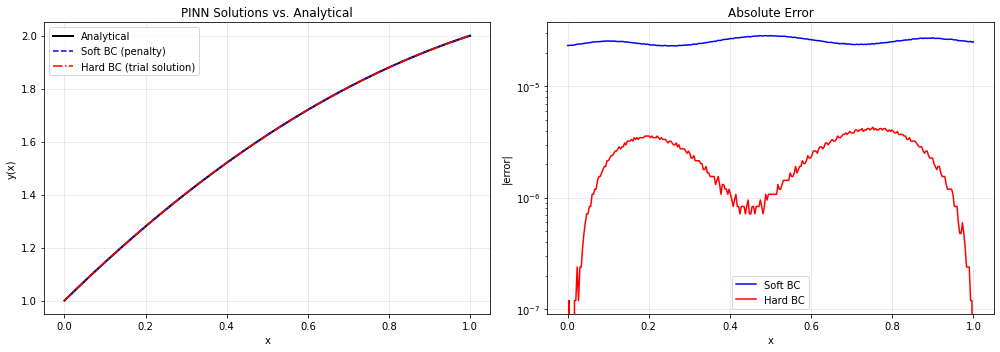
\includegraphics[width=0.97\linewidth]{figures/pinn_softvshard.png}
\end{center}

\begin{center}
{\footnotesize Both fit the solution (left). The difference is the error (right, log scale): the soft-BC run sits near $10^{-3}$ \emphc{including at the endpoints}, while the hard-BC run falls to $10^{-7}$ at the boundary, exact there by construction.}
\end{center}

\vspace{-0.3em}
{\footnotesize\hfill\textbf{Notebook:} \texttt{02\_ODE\_PINN\_SoftVsHardBCs}}
\end{frame}

% --- Finger Exercise: Hard BCs ---
\begin{frame}{\exercisepause{} Finger Exercise: Hard Boundary Conditions}
\begin{exampleblock}{Exercise (5 min)}
Consider the same ODE $u''(x) = -1$ on $[0,1]$ with $u(0)=u(1)=0$.
\begin{enumerate}
    \item Construct a \emphc{hard-BC trial solution} of the form $\hat{u}(x) = B(x) \cdot \mathcal{N}(x; \theta)$, where $B(x)$ enforces both BCs exactly. {\small (Hint: $B$ must vanish at $x=0$ and $x=1$.)}
    \item Verify that $\hat{u}(0) = \hat{u}(1) = 0$ for \emph{any} network output $\mathcal{N}$.
    \item What is the advantage of hard BCs over soft BCs?
\end{enumerate}
\end{exampleblock}
\end{frame}

\begin{frame}{Solution: Hard Boundary Conditions}
\begin{block}{Answer}
\begin{enumerate}
    \item $\hat{u}(x) = x(1-x)\cdot\mathcal{N}(x; \theta)$.  Since $B(x)=x(1-x)$ vanishes at both endpoints, the BCs are satisfied exactly.
    \item $\hat{u}(0)=0\cdot\mathcal{N}(0;\theta)=0$. \quad $\hat{u}(1)=0\cdot\mathcal{N}(1;\theta)=0$. \checkmark\\
    This holds regardless of what $\mathcal{N}$ outputs.
    \item Hard BCs \emphc{eliminate the boundary loss term} entirely, the optimizer only needs to minimize the PDE residual. This reduces the number of hyperparameters ($\lambda$ is gone) and often speeds up convergence.
\end{enumerate}
\end{block}
\end{frame}

% --- Slide 23: 2D Poisson ---
\begin{frame}{Extension to 2D: Poisson Equation}
\textbf{Problem:} $\Delta u = f(x,y)$ on $\Omega = (0,1)^2$ with Dirichlet BCs.

\vspace{0.2em}
\textbf{Manufactured solution:} $u^\star(x,y) = x^2 + y + \sin(\pi x)\sin(\pi y)$.

\vspace{0.4em}
\textbf{Hard BCs via transfinite (Coons-patch) interpolation}, the standard 4-side construction that matches each boundary function exactly along its edge:
\[
\hat{u}(x,y) = A(x,y) + \underbrace{x(1\!-\!x)\,y(1\!-\!y)}_{B(x,y)}\cdot\mathcal{N}_\theta(x,y)
\]

where $A(x,y)$ interpolates boundary data from all four sides:
\[
A = (1\!-\!x)\,g_L(y) + x\,g_R(y) + (1\!-\!y)\,g_B(x) + y\,g_T(x) - \text{corners}
\]

\vspace{0.3em}
\textbf{Laplacian via autograd:}
\[
\Delta\hat{u} = \frac{\partial^2\hat{u}}{\partial x^2} + \frac{\partial^2\hat{u}}{\partial y^2}
\quad\text{(two chains of \texttt{autograd.grad})}
\]
\end{frame}

% --- Slide 24: 2D Results ---
\begin{frame}{2D Poisson: Results}
\begin{center}
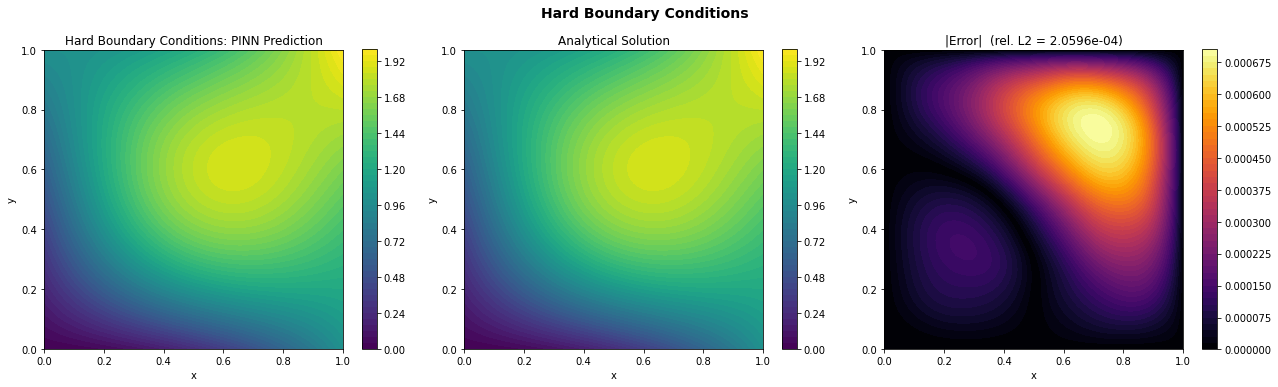
\includegraphics[width=\linewidth]{figures/pinn_poisson2d_hard.png}
\end{center}

\vspace{0.2em}
\begin{center}
{\small Hard-BC PINN, analytical solution, and absolute error. Relative $L^2$ error
$\;\mathbf{2.06\times 10^{-4}}$ against $\;1.36\times 10^{-3}$ for the tuned soft-penalty run:
a \emphc{$6.6\times$} improvement, at one fewer hyperparameter.}
\end{center}

{\small\hfill\textbf{Notebook:} \texttt{03\_PDE\_PINN\_Poisson2D}}
\end{frame}

% --- Slide 25: When to Use Which ---
\begin{frame}{Soft vs.\ Hard BCs: When to Use Which?}
\begin{center}
{\small
\begin{tabular}{p{2.2cm}>{\raggedright\arraybackslash}p{4.5cm}>{\raggedright\arraybackslash}p{4.5cm}}
\toprule
& \textbf{Soft BCs} & \textbf{Hard BCs} \\
\midrule
\textbf{Best for} & Irregular domains, Robin or Neumann BCs & Simple domains, Dirichlet BCs, high accuracy \\
\midrule
\textbf{Pros} & Flexible, easy to implement & Exact BCs, fewer hyperparams, better accuracy \\
\midrule
\textbf{Cons} & $\lambda$ tuning, approximate BCs & Needs analytical $A$, $B$; harder for irregular domains \\
\bottomrule
\end{tabular}
}
\end{center}

\vspace{0.3em}
\begin{block}{Practical recommendation}
Start with \emphc{hard BCs} when the domain and boundary data allow it.
Fall back to \emphc{soft BCs} for complex geometries or mixed boundary types.
\end{block}
\end{frame}

% ============================================================================
% PART IV: ECONOMIC APPLICATIONS --- HJB
% ============================================================================

% --- Slide 26: Section Divider ---
\section{Economic Applications: the HJB Equation}

\begin{frame}{}
\vfill
\begin{center}
{\Huge \textcolor{uzhblue}{\textbf{Part IV}}}\\[12pt]
{\LARGE Economic Applications: The HJB Equation}
\end{center}
\vfill
\end{frame}

% --- Slide 27: HJB Equation ---
\begin{frame}{The Hamilton--Jacobi--Bellman Equation}
\textbf{Generic continuous-time optimization:}
\[
\rho\, V(\x) = \max_{c}\;\bigl\{u(c) + V_{\x}\cdot f(\x, c)\bigr\}
\]

\vspace{0.3em}
\begin{itemize}
    \item $V(\x)$: \emphc{value function} (unknown)
    \item $\rho$: discount rate
    \item $u(c)$: flow utility
    \item $f(\x,c)$: law of motion for state $\x$
    \item $V_{\x} = \nabla V$: gradient of the value function
\end{itemize}

\vspace{0.4em}
\textbf{This is a PDE!} First-order (or second-order with diffusion).

\vspace{0.3em}
$\Rightarrow$ \emphc{Perfect fit for PINNs:} the network approximates $V$, autograd gives $V_{\x}$, and the HJB residual is the loss.
\end{frame}

% --- Slide 28: Cake-Eating Setup ---
\begin{frame}{Cake-Eating Problem: Setup}
\textbf{A household} with wealth $a(t)$ chooses consumption $c(t)$ to maximize lifetime utility:
\[
\max_{\{c(t)\}} \int_0^\infty e^{-\rho t}\,\frac{c(t)^{1-\gamma}}{1-\gamma}\,\mathrm{d}t
\qquad\text{s.t.}\quad \dot{a} = r\,a - c
\]

\textbf{HJB equation:}\quad
$\rho\,V(a) = \max_c\;\bigl\{\frac{c^{1-\gamma}}{1-\gamma} + V'(a)\,(r\,a - c)\bigr\}$

\vspace{0.2em}
\textbf{FOC:} $c^{-\gamma} = V'(a)$ $\;\Rightarrow\;$ $c^\star = \bigl(V'(a)\bigr)^{-1/\gamma}$.

\vspace{0.2em}
\textbf{Analytical solution} (with $\kappa = \frac{\rho - (1-\gamma)r}{\gamma} > 0$):
\[
V^\star(a) = \frac{\kappa^{-\gamma}}{1-\gamma}\,a^{1-\gamma}, \qquad c^\star(a) = \kappa\,a
\]

{\small Parameters: $\gamma = 2$, $\rho = 0.05$, $r = 0.03$ $\;\Rightarrow\;$ $\kappa = 0.04$.}
\end{frame}

% --- Slide 29: PINN for HJB (trial solution, hard BCs) ---
\begin{frame}{PINN for the HJB Equation: Hard-BC Trial Solution}
\textbf{Anchor + mask + scaled MLP.}  Let $x(a) = (a-a_{\min})/(a_{\max}-a_{\min}) \in [0,1]$ and $S$ a value-scale constant:
\[
\hat V(a) \;=\; V^\star(a_{\min}) + x(a)\bigl[V^\star(a_{\max}) - V^\star(a_{\min})\bigr] \;+\; x(a)\bigl(1-x(a)\bigr)\,S\,f_\theta\bigl(x(a)\bigr).
\]
Endpoints are exact \emph{by construction}, so the boundary loss is identically zero and the optimizer focuses on the HJB residual only.

\vspace{0.3em}
\textbf{Consumption} via FOC, $\hat c(a) = (\hat V'(a))^{-1/\gamma}$, with softplus safeguard on $\hat V'$.

\vspace{0.3em}
\textbf{Loss}: only the interior HJB residual remains,
\[
\ell \;=\; \frac{1}{N}\sum_{i}\mathcal{R}(a_i)^2,
\qquad
\mathcal{R}(a) = \rho\hat V - \Bigl[\tfrac{\hat c^{1-\gamma}}{1-\gamma} + \hat V'(ra - \hat c)\Bigr].
\]

\vspace{0.2em}
{\small \emphc{Pedagogical point:} a small MLP plus hard BCs beats a large gated net with a soft-BC penalty, because the boundary term no longer dominates the objective.}
\end{frame}

% --- Slide 30: DGM Architecture (optional / high-D) ---
\begin{frame}{Optional Architecture for High-D PDEs: DGM}
\begin{columns}[T]
\column{0.44\textwidth}
\begin{center}
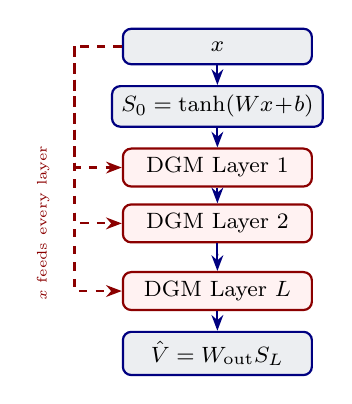
\begin{tikzpicture}[
    block/.style={rectangle, draw=uzhblue, thick, fill=uzhgreylight,
        minimum width=2.4cm, minimum height=0.45cm, font=\footnotesize,
        rounded corners=3pt},
    layer/.style={rectangle, draw=darkred, thick, fill=red!5,
        minimum width=2.4cm, minimum height=0.45cm, font=\footnotesize,
        rounded corners=3pt},
    arr/.style={-{Stealth[length=2mm]}, thick, uzhblue},
    skip/.style={-{Stealth[length=2mm]}, thick, darkred, dashed}
]
    % Input
    \node[block] (inp) {$x$};

    % Initial transform
    \node[block, below=0.25cm of inp] (S0) {$S_0 = \tanh(Wx\!+\!b)$};

    % DGM Layers — stacked to show repetition
    \node[layer, below=0.25cm of S0] (L1) {DGM Layer 1};
    \node[layer, below=0.2cm of L1] (L2) {DGM Layer 2};
    \node[font=\small, text=gray] at ($(L2.south)+(0,-0.18)$) {$\vdots$};
    \node[layer, below=0.35cm of L2] (LL) {DGM Layer $L$};

    % Output
    \node[block, below=0.25cm of LL] (out) {$\hat{V} = W_{\text{out}} S_L$};

    % Vertical arrows
    \draw[arr] (inp) -- (S0);
    \draw[arr] (S0) -- (L1);
    \draw[arr] (L1) -- (L2);
    \draw[arr] (L2) -- (LL);
    \draw[arr] (LL) -- (out);

    % Skip connections from x to every layer
    \draw[skip] (inp.west) -- ++(-0.6,0) |- (L1.west);
    \draw[skip] ([xshift=-0.6cm]inp.west) |- (L2.west);
    \draw[skip] ([xshift=-0.6cm]inp.west) |- (LL.west);

    % Label for skip connections
    \node[font=\tiny, text=darkred, align=center, rotate=90]
        at ([xshift=-1.0cm]L2.west) {$x$ feeds every layer};
\end{tikzpicture}
\end{center}

\column{0.54\textwidth}
\textbf{Deep Galerkin Method}\\
{\small (Sirignano \& Spiliopoulos, 2018)}

\vspace{0.4em}
\begin{itemize}\setlength\itemsep{3pt}
    \item Pays off only in \emphc{higher dimensions}, or where the PDE has sharp features.
    \item The input $x$ enters \emphc{every} layer, not just the first --- that is what resolves steep gradients.
    \item Each layer is \emphc{gated}, LSTM-style; the $x$-skips recall Highway Networks.
\end{itemize}

\vspace{0.4em}
\begin{alertblock}{Not the default choice}
\footnotesize
For the 1D cake problem, the trial-solution MLP of the previous slide is simpler \emph{and} more accurate.
\end{alertblock}
\end{columns}
\end{frame}

% --- Slide 31b: Inside a DGM layer ---
\begin{frame}{Inside a DGM Layer}
\begin{columns}[T]
\column{0.56\textwidth}
{\small $S_\ell\in\R^U$ is the depth-$\ell$ hidden state, initialised as $S_0=\tanh(Wx+b)$; $\odot$ is the Hadamard product; and $Z,G,R$ are sigmoid gates valued in $[0,1]$:}
\vspace{0.2em}
{\small\begin{align*}
Z_\ell &= \sigma(U^z x + W^z S_\ell + b^z)\\
G_\ell &= \sigma(U^g x + W^g S_\ell + b^g)\\
R_\ell &= \sigma(U^r x + W^r S_\ell + b^r)\\
H_\ell &= \tanh(U^h x + W^h (S_\ell \odot R_\ell) + b^h)\\
S_{\ell+1} &= (1 - G_\ell)\odot H_\ell + Z_\ell \odot S_\ell
\end{align*}}

\column{0.42\textwidth}
\begin{block}{Reading the gates}
\footnotesize
$R_\ell$ decides how much of the current state enters the candidate $H_\ell$.\\[4pt]
$G_\ell$ and $Z_\ell$ then blend that candidate against the state being carried forward.\\[4pt]
Every one of them sees $x$ directly.
\end{block}

\vspace{0.4em}
{\footnotesize \textbf{Cost:} four weight matrices per layer instead of one, so roughly $4\times$ the parameters of a plain MLP of the same width.}
\end{columns}
\end{frame}

% --- Slide 31: DGM Code ---
\begin{frame}[fragile]{DGM Implementation (PyTorch)}
\begin{lstlisting}[basicstyle=\scriptsize\ttfamily]
class DGMNet(nn.Module):
    def __init__(self, dim, layers=4, units=64):
        super().__init__()
        self.input = nn.Linear(dim, units)
        self.z  = nn.ModuleList(nn.Linear(dim, units) for _ in range(layers))
        self.wz = nn.ModuleList(nn.Linear(units, units) for _ in range(layers))
        # ... similar for g, r, h gates
        self.out = nn.Linear(units, 1)

    def forward(self, x):
        s = torch.tanh(self.input(x))
        for l in range(len(self.z)):
            z = torch.sigmoid(self.z[l](x) + self.wz[l](s))
            g = torch.sigmoid(self.g[l](x) + self.wg[l](s))
            r = torch.sigmoid(self.r[l](x) + self.wr[l](s))
            h = torch.tanh(self.h[l](x) + self.wh[l](s * r))
            s = (1 - g) * h + z * s
        return self.out(s)
\end{lstlisting}
\end{frame}

% --- Slide 32: HJB Residual Code ---
\begin{frame}[fragile]{HJB Residual Implementation}
\begin{lstlisting}[basicstyle=\footnotesize\ttfamily]
def pde_residual(model, a):
    a.requires_grad_(True)
    V = model(a)                        # value function
    V_a = torch.autograd.grad(          # V'(a) via autograd
        V.sum(), a, create_graph=True)[0].squeeze(-1)

    safe_Va = F.softplus(V_a) + 1e-6   # positivity guard
    c = safe_Va.pow(-1.0 / gamma)       # FOC: optimal c
    u_c = c.pow(1-gamma) / (1-gamma)    # flow utility

    R = rho*V - (u_c + safe_Va*(r*a.squeeze(-1) - c))
    return R                            # HJB residual
\end{lstlisting}

\vspace{0.1em}
{\footnotesize The \texttt{softplus} safeguard prevents $V'(a)^{-1/\gamma}$ from blowing up if $V'(a) \leq 0$ during early training.}
\end{frame}

% --- Slide 33: Cake-Eating Results ---
\begin{frame}{Cake-Eating: the Closed-Form Benchmark}
\begin{columns}[T]
\column{0.48\textwidth}
\begin{center}
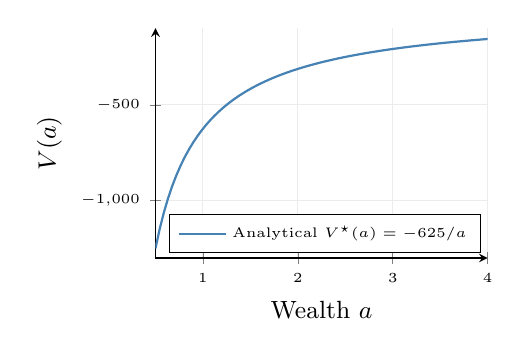
\begin{tikzpicture}
\begin{axis}[
    width=5.8cm, height=4.5cm,
    xlabel={Wealth $a$}, ylabel={$V(a)$},
    xlabel style={font=\small}, ylabel style={font=\small},
    tick label style={font=\tiny},
    xmin=0.5, xmax=4, ymin=-1300, ymax=-100,
    grid=major, grid style={gray!15},
    legend style={font=\tiny, at={(0.98,0.02)}, anchor=south east},
    axis lines=left,
]
    \addplot[thick, softblue, domain=0.5:4, samples=80] {-625/x};
    \addlegendentry{Analytical $V^\star(a) = -625/a$}
\end{axis}
\end{tikzpicture}\\
{\small Value function $V(a)$ (closed form)}
\end{center}

\column{0.48\textwidth}
\begin{center}
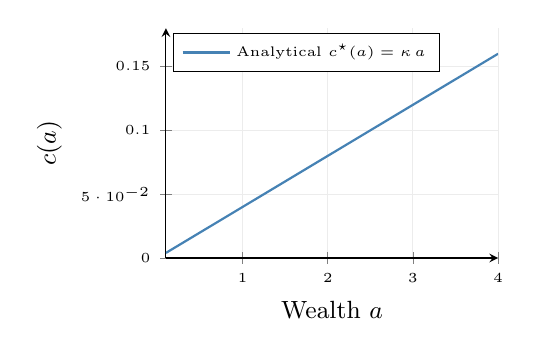
\begin{tikzpicture}
\begin{axis}[
    width=5.8cm, height=4.5cm,
    xlabel={Wealth $a$}, ylabel={$c(a)$},
    xlabel style={font=\small}, ylabel style={font=\small},
    tick label style={font=\tiny},
    xmin=0.1, xmax=4, ymin=0, ymax=0.18,
    grid=major, grid style={gray!15},
    legend style={font=\tiny, at={(0.02,0.98)}, anchor=north west},
    axis lines=left,
]
    \addplot[thick, softblue, domain=0.1:4, samples=80] {0.04*x};
    \addlegendentry{Analytical $c^\star(a) = \kappa\, a$}
\end{axis}
\end{tikzpicture}\\
{\small Consumption policy $c(a)$ (closed form)}
\end{center}
\end{columns}

\vspace{0.1em}
\begin{center}
{\footnotesize These are the \emph{exact} solutions, the target the PINN is scored against. Classroom run: HJB loss $\approx 3\!\times\!10^{-4}$, consumption relative $L^2$ error $\approx 6\!\times\!10^{-3}$. The notebook overlays the fitted $\hat V$ and $\hat c$.}
\end{center}

{\small\hfill\textbf{Notebook:} \texttt{04\_Cake\_Eating\_HJB\_PINN}}
\end{frame}

% --- Slide 34: Extensions ---
\begin{frame}{Extensions: From Cake-Eating to Frontier Models}
\textbf{The PINN/DGM framework scales naturally:}

\vspace{0.3em}
\begin{enumerate}
    \item \textbf{Income risk:} add diffusion $\mathrm{d}a = (ra - c + y)\,\mathrm{d}t + \sigma\,\mathrm{d}W$
    \quad$\Rightarrow$ second-order HJB

    \vspace{0.2em}
    \item \textbf{Aiyagari-type models:} HJB + Kolmogorov Forward Equation
    \quad$\Rightarrow$ coupled PDE system

    \vspace{0.2em}
    \item \textbf{General equilibrium:} prices clear markets
    \quad$\Rightarrow$ hybrid DEQN + PINN

    \vspace{0.2em}
    \item \textbf{High dimensions:} multiple assets, heterogeneous agents
    \quad$\Rightarrow$ no grid needed!
\end{enumerate}

\vspace{0.3em}
{\small See: Achdou et al.\ (2022), Fernandez-Villaverde et al.\ (2024), Gopalakrishna (2024).}
\end{frame}

% ============================================================================
% PART V: BLACK-SCHOLES
% ============================================================================

% --- Slide 35: Section Divider ---
\section{Financial Applications: Black--Scholes}

\begin{frame}{}
\vfill
\begin{center}
{\Huge \textcolor{uzhblue}{\textbf{Part V}}}\\[12pt]
{\LARGE Financial Applications: Black--Scholes}
\end{center}
\vfill
\end{frame}

% --- Slide 36: Black-Scholes PDE ---
\begin{frame}{The Black--Scholes PDE}
\begin{columns}[T]
\column{0.52\textwidth}
\textbf{European call option} ($S$: asset, $K$: strike, $T$: maturity):
\[
\frac{\partial V}{\partial t} + \frac{1}{2}\sigma^2 S^2 \frac{\partial^2 V}{\partial S^2}
+ r S\frac{\partial V}{\partial S} - rV = 0
\]

\textbf{Terminal:} $V(S, T) = \max(S - K, 0)$

\textbf{Boundary conditions:}
\begin{itemize}\setlength{\itemsep}{1pt}
    \item $V(0, t) = 0$
    \item $V(S_{\max}, t) = S_{\max} - Ke^{-r(T-t)}$
\end{itemize}

\column{0.45\textwidth}
\textbf{PINN approach:}
\begin{itemize}\setlength{\itemsep}{2pt}
    \item Network $\mathcal{N}_\theta(S, t) \approx V(S, t)$
    \item Autograd: $V_t$, $V_S$, $V_{SS}$
    \item 4 loss terms:
\end{itemize}

\vspace{0.2em}
{\small
\begin{tabular}{rl}
$\ell_{\text{PDE}}$ & interior residual\\
$\ell_{\text{BC}_0}$ & $V(0,t) = 0$\\
$\ell_{\text{term}}$ & $V(S,T) = \text{payoff}$\\
$\ell_{\text{BC}_{S_{\max}}}$ & far-field BC\\
\end{tabular}
}
\end{columns}
\end{frame}

% --- Slide 37: Black-Scholes Implementation ---
\begin{frame}[fragile]{Black--Scholes PINN: Key Code}
\begin{lstlisting}
def pde_residual(model, S, t):
    S.requires_grad_(True)
    t.requires_grad_(True)
    X = torch.cat([S, t], dim=1)
    V = model(X)

    V_t  = torch.autograd.grad(V, t, (*@\ldots@*))[0]
    V_S  = torch.autograd.grad(V, S, (*@\ldots@*))[0]
    V_SS = torch.autograd.grad(V_S, S, (*@\ldots@*))[0]

    # Black-Scholes PDE residual
    res = V_t + 0.5*sigma**2*S**2*V_SS + r*S*V_S - r*V
    return res
\end{lstlisting}

\vspace{0.1em}
{\small\textbf{Loss:}
\[
\ell = \text{MSE}(\text{res}) + \text{MSE}(V|_{S=0}) + \text{MSE}(V|_{t=T} - \text{payoff}) + \text{MSE}(V|_{S_{\max}} - \text{target})
\]
}
\end{frame}

% --- Slide 38: Black-Scholes Results ---
\begin{frame}{Black--Scholes: the Closed-Form Benchmark}
\begin{columns}[T]
\column{0.55\textwidth}
\begin{center}
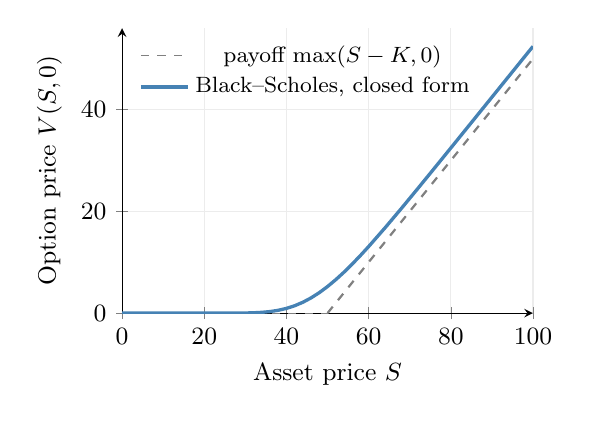
\begin{tikzpicture}
\begin{axis}[
    width=6.8cm, height=5.2cm,
    xlabel={Asset price $S$}, ylabel={Option price $V(S, 0)$},
    xlabel style={font=\small}, ylabel style={font=\small},
    tick label style={font=\small},
    xmin=0, xmax=100, ymin=0, ymax=56,
    grid=major, grid style={gray!15},
    legend style={font=\footnotesize, at={(0.02,0.98)}, anchor=north west, draw=none, fill=none},
    axis lines=left,
]
    \addplot[thick, gray, dashed, domain=0:100, samples=2, forget plot] coordinates {(50,0) (100,50)};
    \addplot[gray, dashed, domain=0:50, samples=2] coordinates {(0,0) (50,0)};
    \addlegendentry{payoff $\max(S-K,0)$}
    \addplot[very thick, softblue] coordinates {
      (0,0.000) (10,0.000) (20,0.000) (24,0.001) (26,0.002) (28,0.009)
      (30,0.027) (32,0.069) (34,0.154) (36,0.307) (38,0.556) (40,0.930)
      (42,1.451) (44,2.138) (46,2.997) (48,4.029) (50,5.225) (52,6.571)
      (54,8.049) (56,9.640) (58,11.324) (60,13.085) (64,16.772) (68,20.605)
      (72,24.520) (76,28.477) (80,32.457) (86,38.444) (92,44.440) (100,52.439)};
    \addlegendentry{Black--Scholes, closed form}
\end{axis}
\end{tikzpicture}
\end{center}

\column{0.42\textwidth}
{\small
\textbf{Parameters:} $K = 50$, $T = 1$, $r = 0.05$, $\sigma = 0.2$, $S_{\max} = 100$.

\vspace{0.2em}
\textbf{Network:} 3 hidden layers, 64 units, $\tanh$; 2{,}500 Adam epochs, then 300 L-BFGS iterations.

\vspace{0.3em}
The gap between the curves is the \emphc{time value}: at the money the option is worth $5.23$, not $0$.

\vspace{0.3em}
Against this benchmark the notebook reports max absolute error $\approx 0.13$, mean $\approx 0.04$, and plots the PINN overlay.
}
\end{columns}

\vspace{0.2em}
{\small\hfill\textbf{Notebook:} \texttt{05\_Black\_Scholes\_PINN}}
\end{frame}

% ============================================================================
% PART VI: PATHOLOGIES, HANDS-ON, AND WRAP-UP
% ============================================================================

\section{When to Use One, and What Goes Wrong}

% --- Slide 38b: Section Divider ---
\begin{frame}{}
\vfill
\begin{center}
{\Huge \textcolor{uzhblue}{\textbf{Part VI}}}\\[12pt]
{\LARGE When to Use One, and What Goes Wrong}
\end{center}
\vfill
\end{frame}

% --- Slide 38b2: Honest comparison against a classical solver ---
\begin{frame}{Should You Use a PINN at All?}
\textbf{On a 1D problem, finite differences win. Outright.}

\vspace{0.4em}
\begin{columns}[T]
\column{0.52\textwidth}
{\small Notebook \texttt{07} solves the same partial-equilibrium HJB both ways:}
\begin{itemize}\setlength\itemsep{2pt}
    \item \emphc{Upwind implicit FD}: 13 iterations on a 500-point grid, then the error is whatever the discretization gives you --- and you can shrink it by refining.
    \item \emphc{PINN}: thousands of epochs to reach $10^{-3}$--$10^{-2}$, with no comparable knob.
\end{itemize}

\vspace{0.5em}
{\small Anyone selling you PINNs as a universal replacement for a grid solver is overselling.}

\vspace{0.3em}

\column{0.45\textwidth}
\begin{block}{Where the trade flips}
\footnotesize
A tensor grid needs $n^d$ points. At $n=50$:\\[3pt]
\begin{tabular}{@{}rl@{}}
$d=1$ & $50$ \\
$d=2$ & $2{,}500$ \\
$d=4$ & $6.3$ million \\
$d=6$ & $1.6\times10^{10}$ \\
\end{tabular}\\[4pt]
Collocation cost is set by the \emph{sample size you choose}, not by $d$.
\end{block}
\end{columns}

\vspace{0.4em}
{\footnotesize \emphc{Use a PINN when} the state space is high-dimensional, the domain is irregular, there are many discrete states, or you need the solution \emph{and} its derivatives as a differentiable object. Otherwise, use the grid.}
\end{frame}

% --- Slide 38b3: The other half of Raissi et al. ---
\begin{frame}{The Other Half: Inverse Problems}
\textbf{So far the PDE was known and we solved it.} Raissi et al.\ (2019) also treat the reverse.

\vspace{0.4em}
\begin{columns}[T]
\column{0.48\textwidth}
\begin{block}{Forward problem}
\small
Parameters $\mu$ given, solve for $u$.\\[4pt]
$\ell(\theta) = \|\mathcal{D}_\mu[\mathcal{N}_\theta]\|^2 + \text{BCs}$
\end{block}

\column{0.48\textwidth}
\begin{alertblock}{Inverse problem}
\small
Some data on $u$ observed, solve for $u$ \emph{and} $\mu$.\\[4pt]
$\ell(\theta,\mu) = \|\mathcal{D}_\mu[\mathcal{N}_\theta]\|^2 + \|\mathcal{N}_\theta - u^{\text{obs}}\|^2$
\end{alertblock}
\end{columns}

\vspace{0.5em}
\begin{itemize}\setlength\itemsep{3pt}
    \item $\mu$ is just \emphc{another set of trainable parameters}: one extra tensor, same optimizer, same loop.
    \item In economics $\mu$ is a \emphc{structural parameter} --- risk aversion, a discount rate, an adjustment cost --- and the data term is a moment condition.
    \item This is estimation and solution in \emphc{one} optimization, rather than a solver nested inside an estimation loop.
\end{itemize}

\vspace{0.3em}
{\footnotesize Connects directly to the deep-surrogate approach to structural estimation from Day 1.}
\end{frame}

% --- Slide 38c: When PINNs fail — the multi-component loss again ---
\begin{frame}{When PINNs Fail: the Multi-Component Loss, Again}
\textbf{The soft-BC loss is a weighted sum of residuals that live at different scales:}
\[
\ell_\theta = \underbrace{\lambda_{\text{pde}}\,\ell_{\text{pde}}}_{\text{interior}}
\;+\; \underbrace{\lambda_{\text{bc}}\,\ell_{\text{bc}}}_{\text{boundary}}
\;+\; \underbrace{\lambda_{\text{ic}}\,\ell_{\text{ic}}}_{\text{initial}}
\]

\vspace{0.5em}
\begin{columns}[T]
\column{0.50\textwidth}
\textbf{This is exactly the Day 1 pathology.}
\begin{itemize}\setlength\itemsep{2pt}
    \item A residual carrying $S^2\partial_{SS}V$ is not in the same units as one carrying $V$ itself.
    \item The largest-scale component captures the gradient; the others are effectively ignored.
    \item Adaptive weights cannot close a gap of several orders of magnitude.
\end{itemize}

\column{0.47\textwidth}
\begin{block}{What to do, in order}
\small
\textbf{1.}~\emphc{Non-dimensionalize} first --- rescale so every residual is $O(1)$.\\[3pt]
\textbf{2.}~Enforce \emphc{structurally} where you can: a hard-BC trial solution deletes $\ell_{\text{bc}}$ from the sum.\\[3pt]
\textbf{3.}~Only then reach for adaptive weights.
\end{block}
\end{columns}

\vspace{0.3em}
{\footnotesize On Day 1 this bought $\approx 110\times$ over equal weighting, where the best adaptive scheme managed $2\times$ (\texttt{02\_DEQN.pdf}, Part IV). See Wang, Teng \& Perdikaris (2021).}
\end{frame}

% --- Slide 38d: Hands-on ---
\begin{frame}{Hands-On: What to Run}
\textbf{All seven notebooks are PyTorch, CPU-only, and self-contained.}\\[2pt]
{\footnotesize Run them on \href{https://nuvolos.cloud}{nuvolos.cloud} --- no local setup needed.}

\vspace{0.4em}
\textbf{Start here, in this order:}
\begin{itemize}\setlength\itemsep{1pt}
    \item The simplest possible PINN: $y''=-1$ with zero BCs \hfill{\footnotesize\texttt{01}}
    \item Soft penalty vs.\ hard trial solution --- the core choice \hfill{\footnotesize\texttt{02}}
    \item The first economic application: the cake-eating HJB \hfill{\footnotesize\texttt{04}}
\end{itemize}

\vspace{0.3em}
\textbf{Then, at your own pace:}
\begin{itemize}\setlength\itemsep{1pt}
    \item 2D Poisson: hard BCs by transfinite interpolation \hfill{\footnotesize\texttt{03}}
    \item Black--Scholes, Greeks for free by autodiff \hfill{\footnotesize\texttt{05}}
    \item PE HJB with discrete income, against an FD benchmark \hfill{\footnotesize\texttt{07}}
\end{itemize}

\vspace{0.1em}
\begin{exampleblock}{Build one yourself (\textasciitilde30 min)}
\footnotesize
Notebook \texttt{06} is a fill-in-the-blank exercise: a PINN for $u''+u=0$ on $[0,\pi]$, solution $\sin(x)$. Solutions follow each task in the same file.
\end{exampleblock}
\end{frame}

% --- Slide 39: Summary ---
\begin{frame}{Summary and Key Takeaways}
\begin{columns}[T]
\column{0.32\textwidth}
\begin{block}{Method}
\centering\small
\vspace{0.2em}
PINNs embed \emphc{differential equations} directly into the neural network loss function via \emphc{automatic differentiation}.
\vspace{0.2em}
\end{block}

\column{0.32\textwidth}
\begin{block}{Boundary Conditions}
\centering\small
\vspace{0.2em}
\emphc{Hard BCs} (trial solutions) eliminate tuning and ensure exact satisfaction. Use \emphc{soft BCs} for complex domains.
\vspace{0.2em}
\end{block}

\column{0.32\textwidth}
\begin{block}{Applications}
\centering\small
\vspace{0.2em}
HJB equations, Black--Scholes, and any continuous-time model. Scales to \emphc{high dimensions} without grids.
\vspace{0.2em}
\end{block}
\end{columns}

\vspace{0.6em}
\textbf{From DEQNs to PINNs:}
\begin{itemize}
    \item \emphc{Same philosophy:} economic/financial equations \emph{are} the loss
    \item \emphc{New ingredient:} \texttt{torch.autograd.grad} for derivatives of $\mathcal{N}_\theta$
    \item \emphc{Broader scope:} any PDE, not just algebraic equilibrium conditions
\end{itemize}
\end{frame}

% --- Slide 40: Questions ---
\begin{frame}{}
\begin{columns}[c]
\column{0.45\textwidth}
\begin{center}
{\Huge \textcolor{uzhblue}{\textbf{Questions?}}}

\vspace{1.0cm}
{\large Simon Scheidegger}\\[4pt]
{\small HEC, University of Lausanne}\\[4pt]
\url{https://sischei.github.io}

\vspace{0.6cm}
{\small Materials:~~\href{https://github.com/sischei/summer-school-AI-for-economics-and-finance-2026}{github.com/sischei/summer-school-AI-\ldots-2026}}
\end{center}

\column{0.45\textwidth}
\begin{center}
\textbf{Companion Notebooks:}\\[8pt]
{\small
\begin{tabular}{rl}
01 & ODE PINN (zero BCs) \\
02 & Soft vs.\ hard BCs \\
03 & 2D Poisson \\
04 & Cake-eating HJB \\
05 & Black--Scholes \\
06 & Exercise: build a PINN \\
07 & PE HJB: FD vs.\ PINN \\
\end{tabular}
}

\vspace{0.7cm}
\textbf{Next up:}\\[6pt]
{\large Deep Learning for}\\
{\large Continuous-Time Models}\\[6pt]
{\small 11:00--12:30~~$\cdot$~~Yucheng Yang}
\end{center}
\end{columns}
\end{frame}

\end{document}
